\chapter{Graphically Solving Linear Programs}
\todoChapter{ {\color{gray}50\% complete. Goal 80\% completion date: July 20}\\
Notes: }
\begin{outcome}
\begin{enumerate}
\item[A.] Learn how to plot the feasible region and the objective function.
\item[B.] Identify and compute extreme points of the feasible region.
\item[C.] Find the optimal solution(s) to a linear program graphically.
\item[D.] Classify the type of result of the problem as infeasible, unbounded, unique optimal solution, or infinitely many optimal solutions.
\end{enumerate}
\end{outcome}
\begin{resource}
\begin{itemize}
\item \href{https://www.youtube.com/watch?v=K7TL5NMlKIk&ab_channel=Dr.TreforBazett}{Youtube! - Modeling with Linear Programming - Watch 4:20 - End}
\item \href{https://www.youtube.com/watch?v=E72DWgKP_1Y&t=1014s&ab_channel=TomS}{Youtube! - Watch 1:43 - 3:43}
\end{itemize}
\end{resource}

Linear Programs (LP's) with two variables can be solved graphically by plotting the feasible region along with the level curves of the objective function.\footnote{Special thanks to Joshua Emmanual and Christopher Griffin for sharing their content to help put this section together. Proper citations and referenes are forthcoming.} We will show that we can find a point in the feasible region that maximizes the objective function using the level curves of the objective function.

We will begin with an easy example that is bounded and investigate the structure of the feasible region.  We will then explore other examples.

%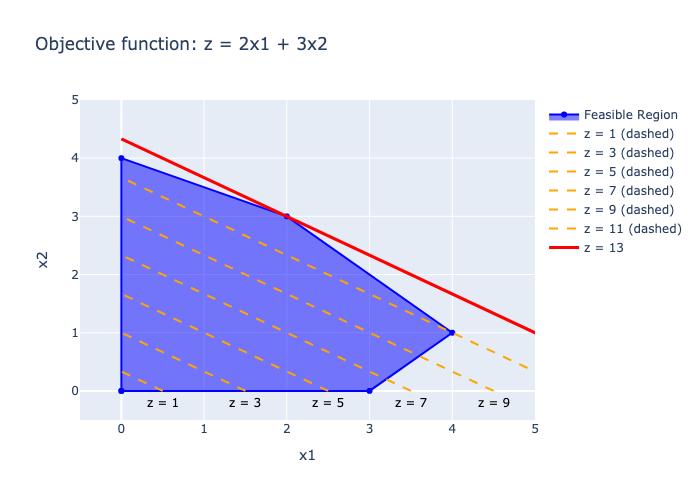
\includegraphics[width = 0.3\textwidth]{Figures/LP-graphical2.png}
%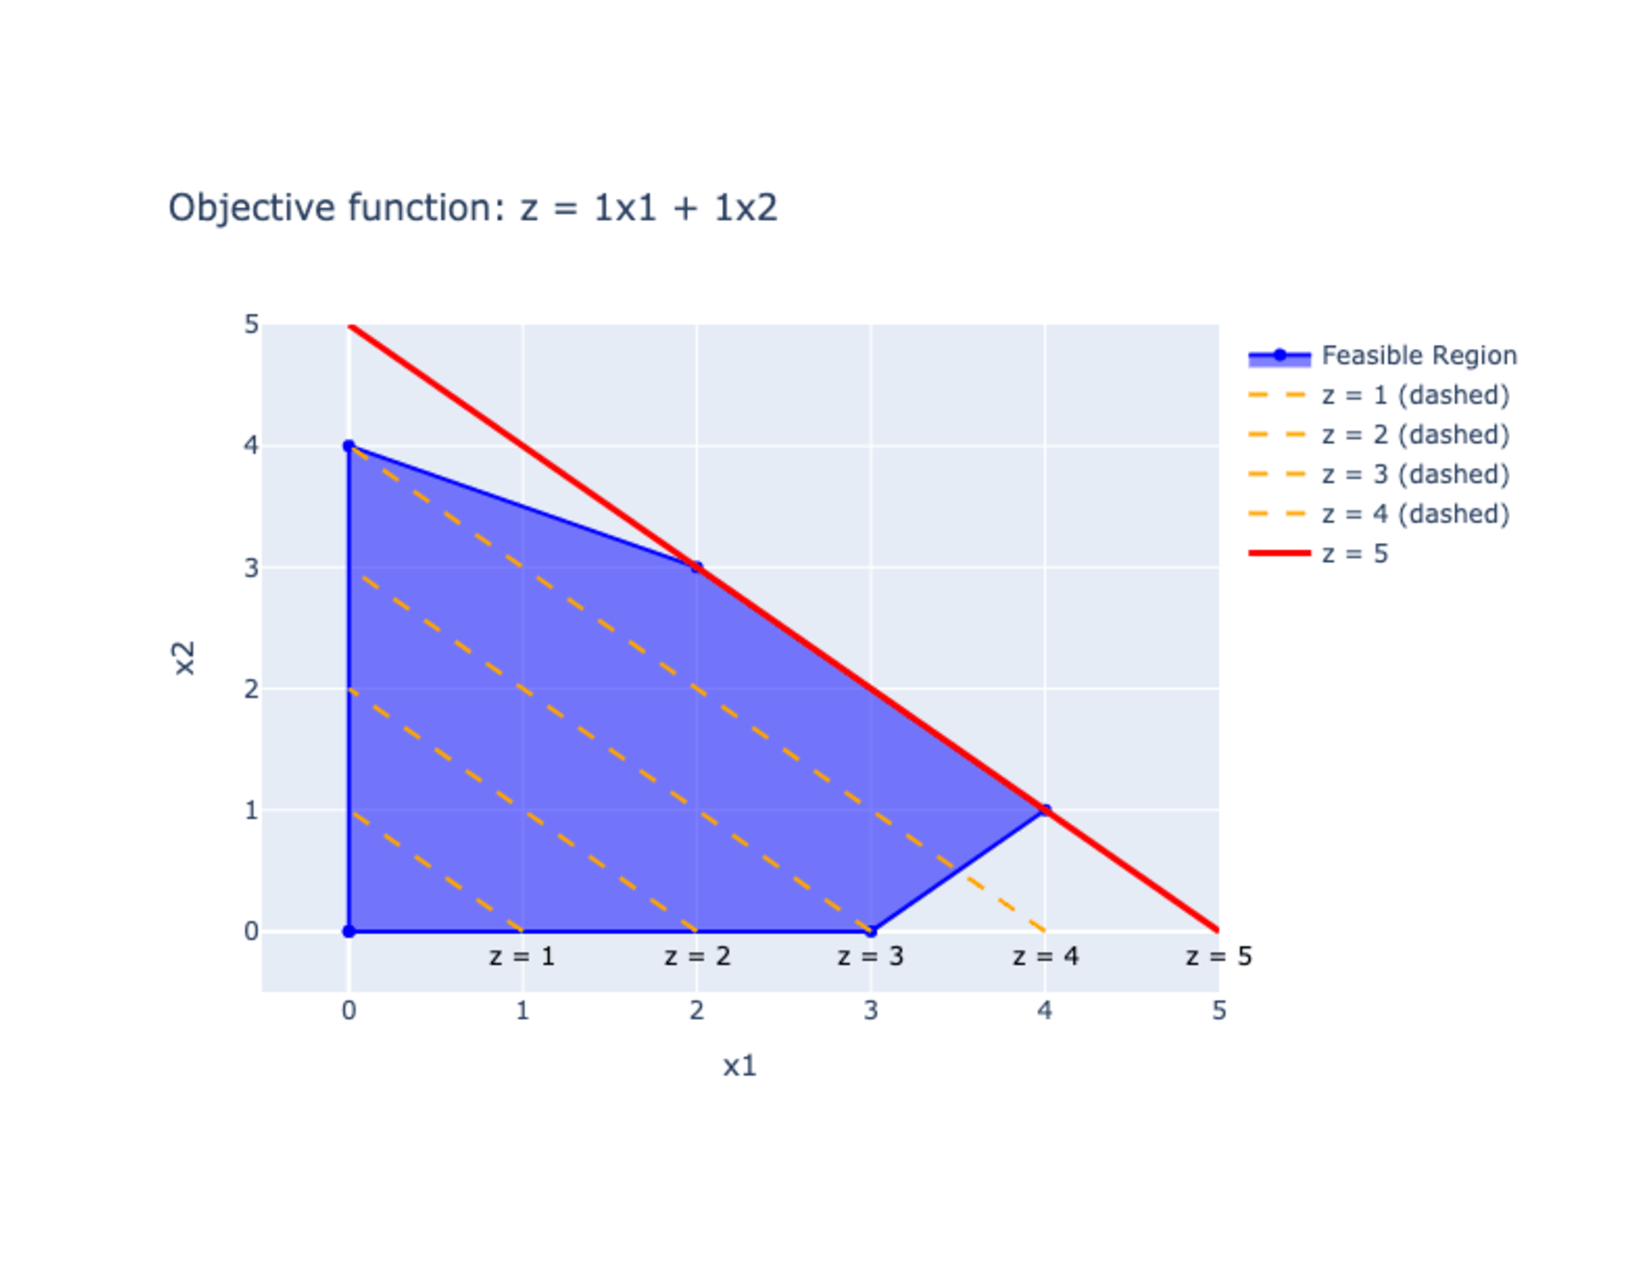
\includegraphics[width = 0.3\textwidth]{Figures/LP-graphical2}
%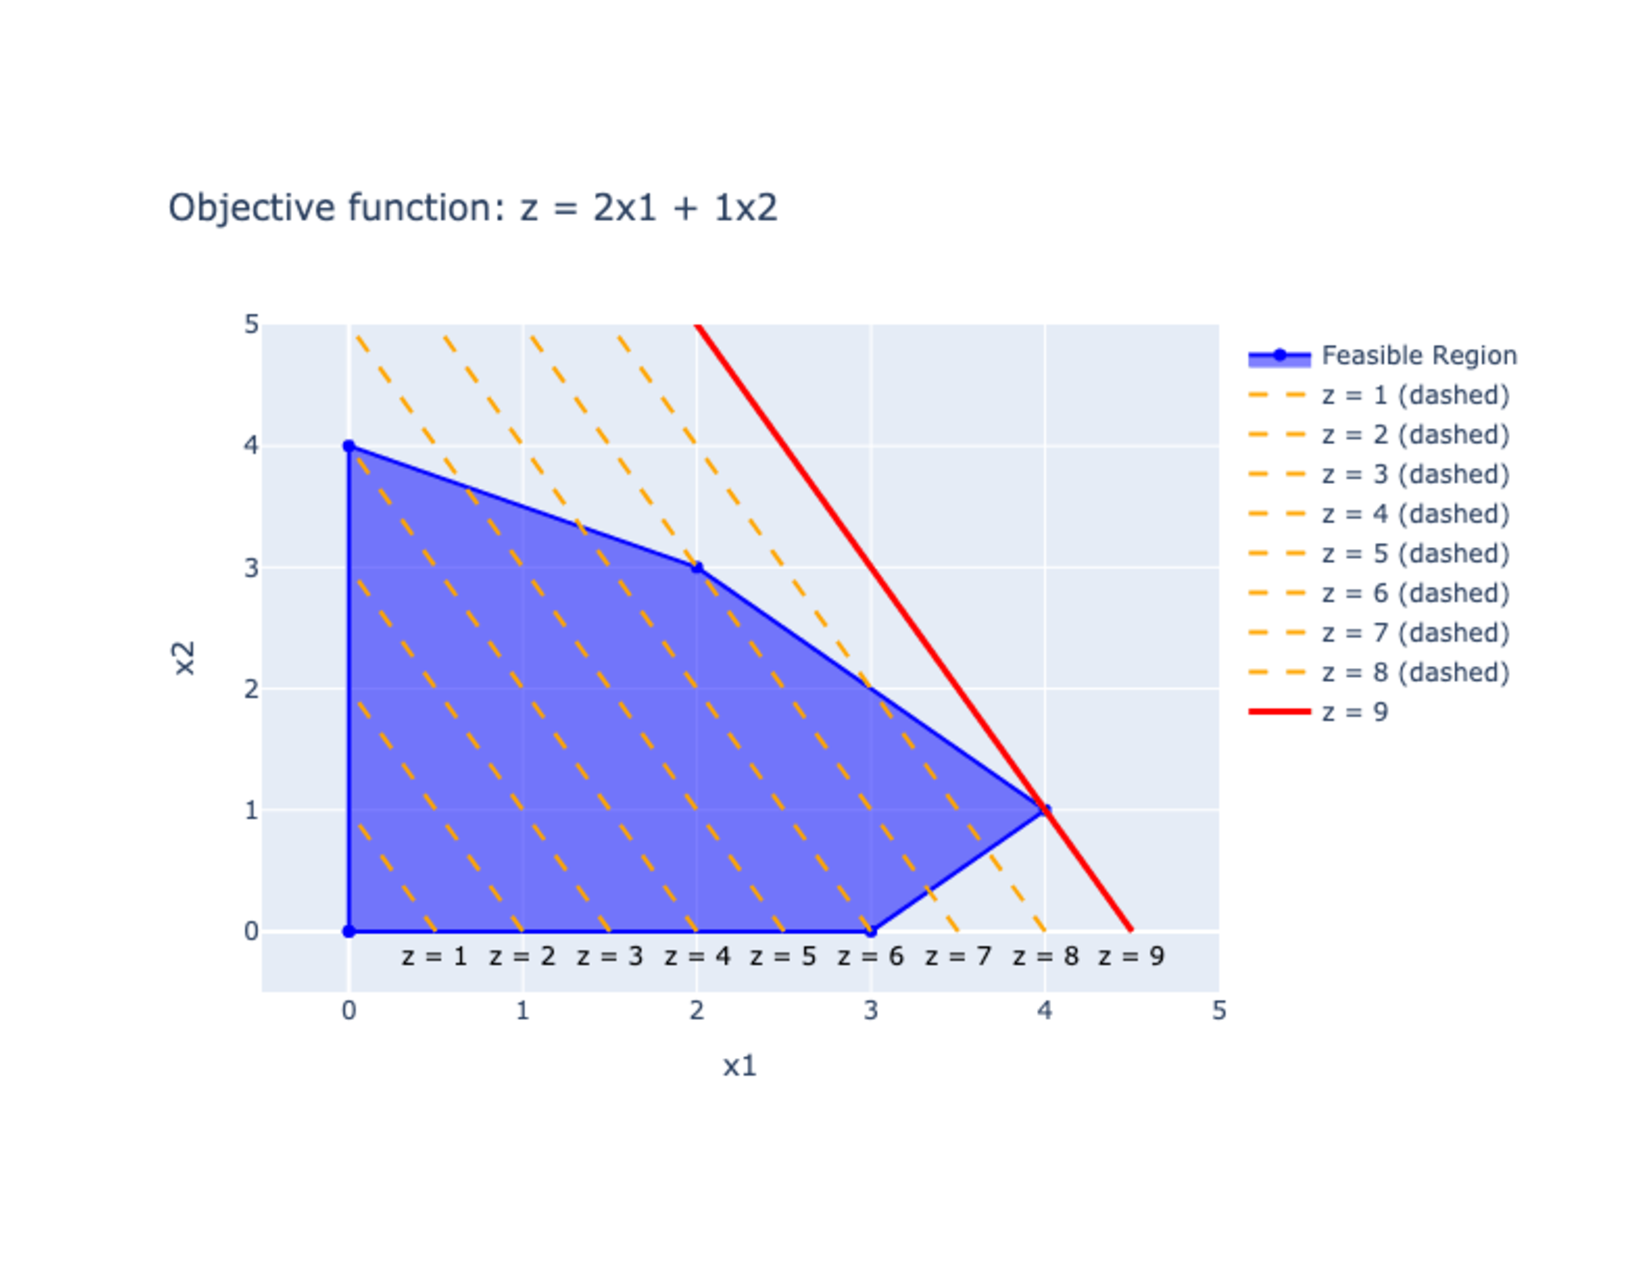
\includegraphics[width = 0.3\textwidth]{Figures/LP-graphical3}



\section{Nonempty and Bounded Problem}
\todoSection{ 20\% complete. Goal 80\% completion date: August 20\\
Notes: Need to work on this section.}
Consider the problem
\begin{align*}
\max \quad & 2 x_1+5 x_2 \\
\text { s.t. } \quad 
&x_1+2 x_2 \leq 16 \\
&5 x_1+3 x_2 \leq  45 \\
&x_1, x_2  \geq 0
\end{align*}

We want to start by plotting the \emph{feasible region}, that is, the set points $(x_1,x_2)$ that satisfy all the constraints. 

We can plot this by first plotting the four lines
\begin{itemize}
\item $x_1+2 x_2 = 16$
\item $5 x_1+3 x_2 = 45$
\item $x_1 = 0$
\item $x_2= 0$
\end{itemize}
and then shading in the side of the space cut out by the corresponding inequality.

\begin{figure}[h!]
\begin{center}
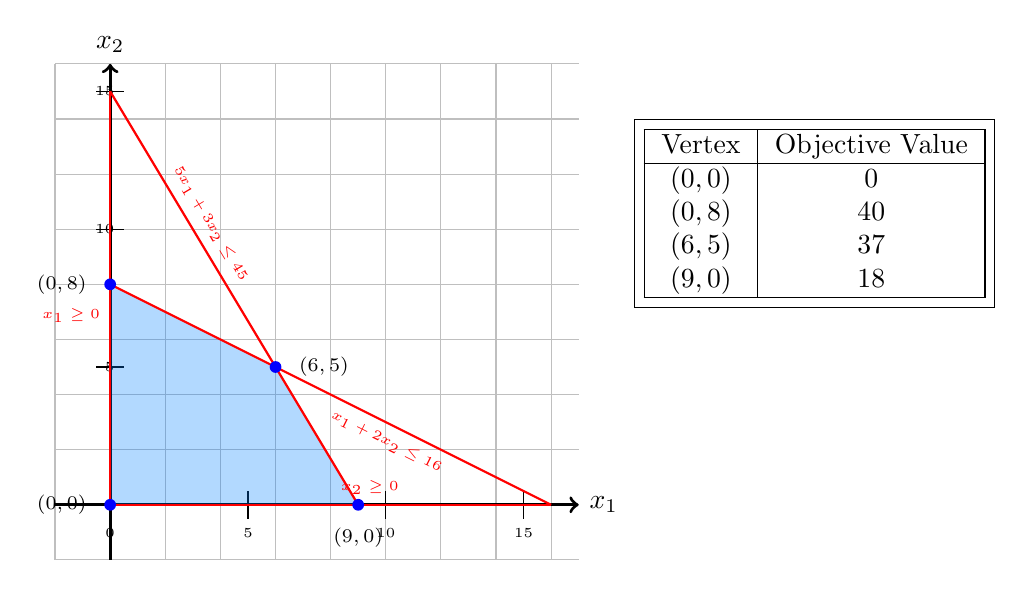
\begin{tikzpicture}[scale = 0.35]
    % Grid and axes
    \draw[gray!50, thin, step=2] (-2,-2) grid (17,16);
    \draw[very thick,->] (-2,0) -- (17,0) node[right] {$x_1$};
    \draw[very thick,->] (0,-2) -- (0,16) node[above] {$x_2$};

    % Axis labels
    \foreach \x in {0,5,10,15} \draw (\x,0.5) -- (\x,-0.5) node[below] {\tiny\x};
    \foreach \y in {0,5,10,15} \draw (-0.5,\y) -- (0.5,\y) node[left] {\tiny\y};

    % Shaded feasible region
    \fill[blue!50!cyan,opacity=0.3] (0,0) -- (0,8) -- (6,5) -- (9,0) -- cycle;

    % Constraint lines
    \draw[red,thick] (0,8) -- node[below right,sloped] {\tiny$x_1 + 2x_2 \leq 16$} (16,0);
    \draw[red,thick] (0,15) -- node[above left,sloped] {\tiny$5x_1 + 3x_2 \leq 45$} (9,0);
    \draw[red,thick] (0,0) -- node[below left] {\tiny$x_1 \geq 0$} (0,15);
    \draw[red,thick] (0,0) -- node[above right] {\tiny$x_2 \geq 0$} (16,0);

    % Vertices
    \node[blue] at (0,0) [circle,fill,inner sep=1.5pt]{};
    \node[blue] at (0,8) [circle,fill,inner sep=1.5pt]{};
    \node[blue] at (6,5) [circle,fill,inner sep=1.5pt]{};
    \node[blue] at (9,0) [circle,fill,inner sep=1.5pt]{};

    % Labels for vertices
    \node[black,anchor=east] at (-0.5,0) {\scriptsize$(0,0)$};
    \node[black,anchor=east] at (-0.5,8) {\scriptsize$(0,8)$};
    \node[black,anchor=west] at (6.5,5) {\scriptsize$(6,5)$};
    \node[black,anchor=north] at (9,-0.5) {\scriptsize$(9,0)$};
% Table within the TikZ picture
    \node[draw,fill=white,anchor=north west] at (19,14) {
        \begin{tabular}{|c|c|}
        \hline
        Vertex & Objective Value \\
        \hline
        $(0,0)$ & $0$ \\
        $(0,8)$ & $40$ \\
        $(6,5)$ & $37$ \\
        $(9,0)$ & $18$ \\
        \hline
        \end{tabular}
    };
\end{tikzpicture}
\end{center}
\caption{\href{https://www.desmos.com/calculator/j1li4l7lcv}{Desmos: Interactive plot!}}
\end{figure}


%\begin{center}
%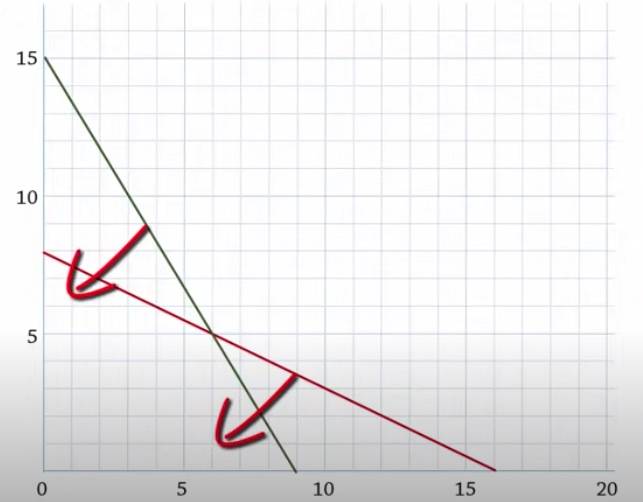
\includegraphics[scale = 0.4]{screenshots/example0-inequalities}
%\end{center}

The resulting feasible region can then can be shaded in as the region that satisfies all the inequalties.

%\begin{center}
%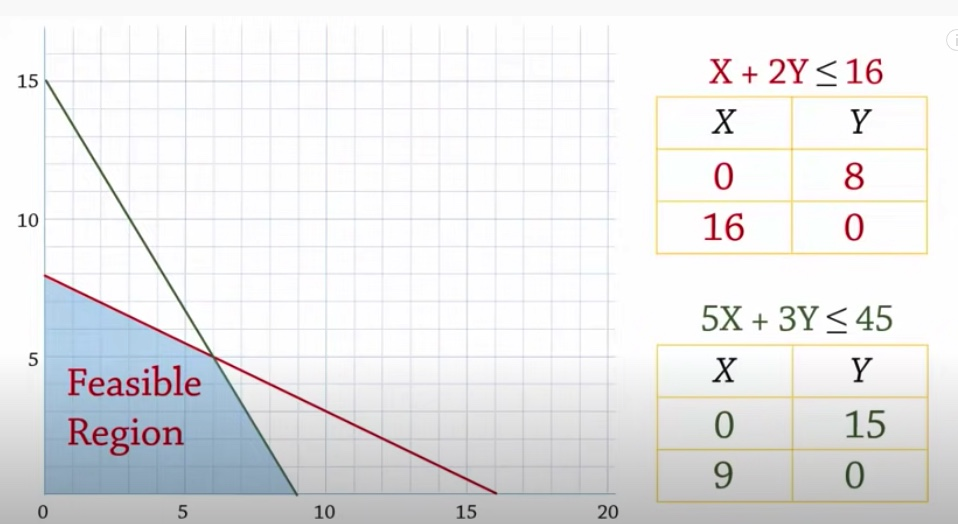
\includegraphics[scale = 0.4]{screenshots/example0-feasible-region}
%\end{center}

Notice that the feasible region is nonempty (it has points that satisfy all the inequalities) and also that it is bounded (the feasible points dont continue infinitly in any direction).

We want to identify the \emph{extreme points} (i.e., the corners) of the feasible region. 
Understanding these points will be critical to understanding the optimal solutions of the model.
Notice that all extreme points can be computed by finding the intersection of 2 of the lines.   But!  Not all intersections of any two lines are feasible.  

We will later use the terminology \emph{basic feasible solution} for an extreme point of the feasible region, and \emph{basic solution} as a point that is the intersection of 2 lines, but is actually infeasible (does not satisfy all the constraints).

%\begin{center}
%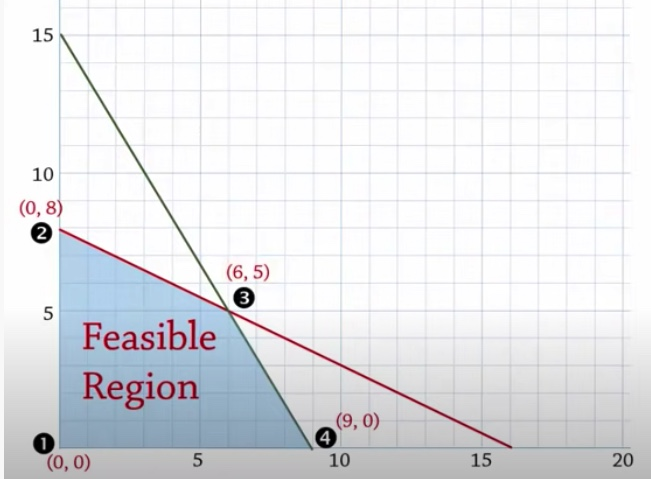
\includegraphics[scale = 0.4]{screenshots/example0-extreme-points}
%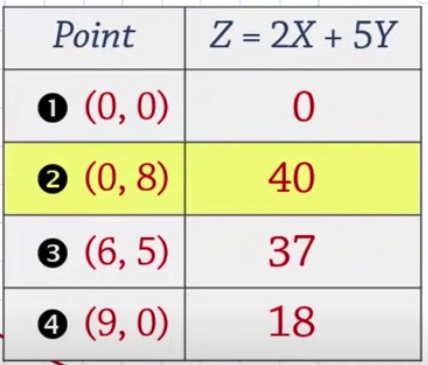
\includegraphics[scale = 0.4]{screenshots/example0-extreme-point-solutions}
%\end{center}

\begin{theorem}{Optimal Solution at a Vertex}{optimalextremepoint}
If the feasible region of the linear program is nonempty and bounded, then there exists an optimal solution at vertex of the feasible region.
\label{thm:optimalextremepoint}
\end{theorem}

This theorem implies the following algorithm.
\begin{algorithm}[H]
\caption{Enumerate Vertices Algorithm for Solving a Linear Programming Problem}
\label{alg:EnumerateVertices}
\begin{enumerate}
    \item \textbf{Identify the Feasible Region:} 
    Determine the set of constraints defining the feasible region in the problem.
    \item \textbf{Enumerate Vertices:}
    Find all the vertices (corner points) of the feasible region. This can be done by solving pairs of constraint equations to find their intersections, keeping only those that satisfy all constraints.
    \item \textbf{Compute Objective Values:} 
    Evaluate the objective function at each vertex of the feasible region.
    \item \textbf{Compare Objective Values:} 
    For a maximization problem, identify the vertex with the highest objective value. For a minimization problem, identify the vertex with the lowest objective value.
    \item \textbf{Determine the Optimal Solution:} 
    The vertex with the optimal objective value is the solution to the linear programming problem.
\end{enumerate}
\end{algorithm}


We will explore why Theorem~\ref{thm:optimalextremepoint} is true, and also what happens when the feasible region does not satisfy the assumtions of either nonempty or bounded.  


\section{Graphical Approach}
We illustrate the idea first using the problem from Example \ref{ex:ToyMaker}.  In a later section, we will formalize the mathematics to explain this result.





\begin{figure}[H] 
\centering
\begin{center}
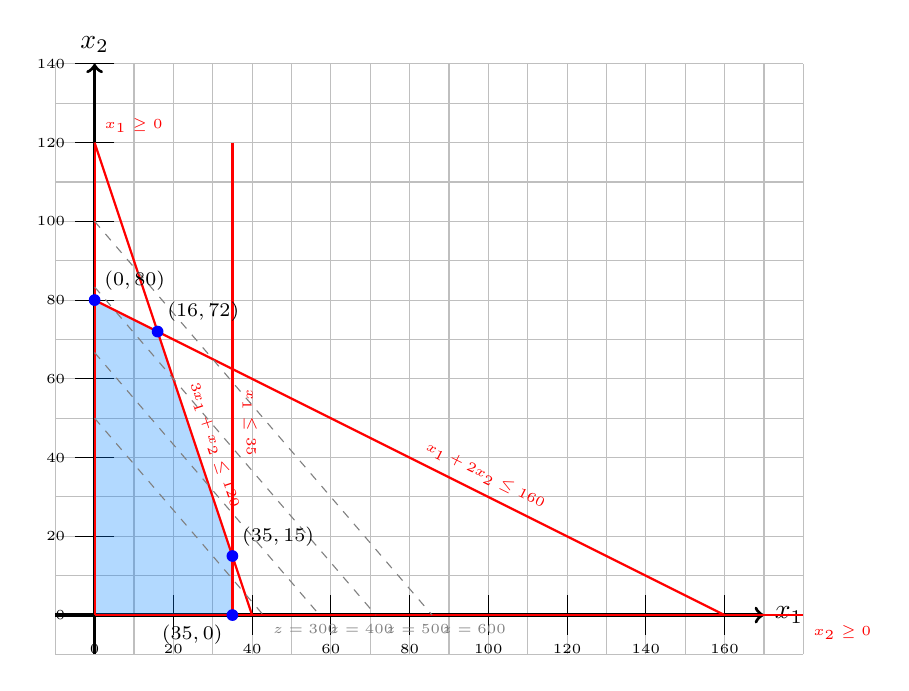
\begin{tikzpicture}[scale=0.05]
    % Grid and axes
    \draw[gray!50, thin, step=10] (-10,-10) grid (180,140);
    \draw[very thick,->] (-10,0) -- (170,0) node[right] {$x_1$};
    \draw[very thick,->] (0,-10) -- (0,140) node[above] {$x_2$};

    % Axis labels
    \foreach \x in {0,20,...,160} \draw (\x,5) -- (\x,-5) node[below] {\tiny\x};
    \foreach \y in {0,20,...,140} \draw (5,\y) -- (-5,\y) node[left] {\tiny\y};

    % Feasible region vertices
    \fill[blue!50!cyan,opacity=0.3] 
        (0,0) -- (0,80) -- (16,72) -- (35,15) -- (35,0) -- cycle;

    % Constraint lines
    \draw[red,thick] (0,120/1) --  node[above right, sloped] {\tiny $3x_1 + x_2 \leq 120$}(120/3,0);
    \draw[red,thick] (0,160/2) --  node[above right, sloped] {\tiny $x_1 + 2x_2 \leq 160$}(160,0);
    \draw[red,thick] (35,120) --  node[above right, sloped] {\tiny $x_1 \leq 35$}(35,0);
    \draw[red,thick] (0,0) -- (180,0) node[below right] {\tiny $x_2 \geq 0$};
    \draw[red,thick] (0,0) -- (0,120) node[above right] {\tiny $x_1 \geq 0$};

    % Objective function contours
    \draw[dashed,gray] (0,600/6) -- (600/7,0) node[below right] {\tiny $z = 600$};
    \draw[dashed,gray] (0,300/6) -- (300/7,0) node[below right] {\tiny $z = 300$};
    \draw[dashed,gray] (0,400/6) -- (400/7,0) node[below right] {\tiny $z = 400$};
    \draw[dashed,gray] (0,500/6) -- (500/7,0) node[below right] {\tiny $z = 500$};

    % Labels for vertices
    \node[blue] at (0,80) [circle,fill,inner sep=1.5pt]{};
    \node[blue] at (16,72) [circle,fill,inner sep=1.5pt]{};
    \node[blue] at (35,15) [circle,fill,inner sep=1.5pt]{};
    \node[blue] at (35,0) [circle,fill,inner sep=1.5pt]{};

    % Vertex coordinates
    \node[black,anchor=south west] at (0,80) {\scriptsize $(0,80)$};
    \node[black,anchor=south west] at (16,72) {\scriptsize $(16,72)$};
    \node[black,anchor=south west] at (35,15) {\scriptsize $(35,15)$};
    \node[black,anchor=north east] at (35,0) {\scriptsize $(35,0)$};

    % Objective function label
    %\node[gray] at (30,140) {\tiny $7x_1 + 6x_2 = z$};
\end{tikzpicture}
\end{center}
%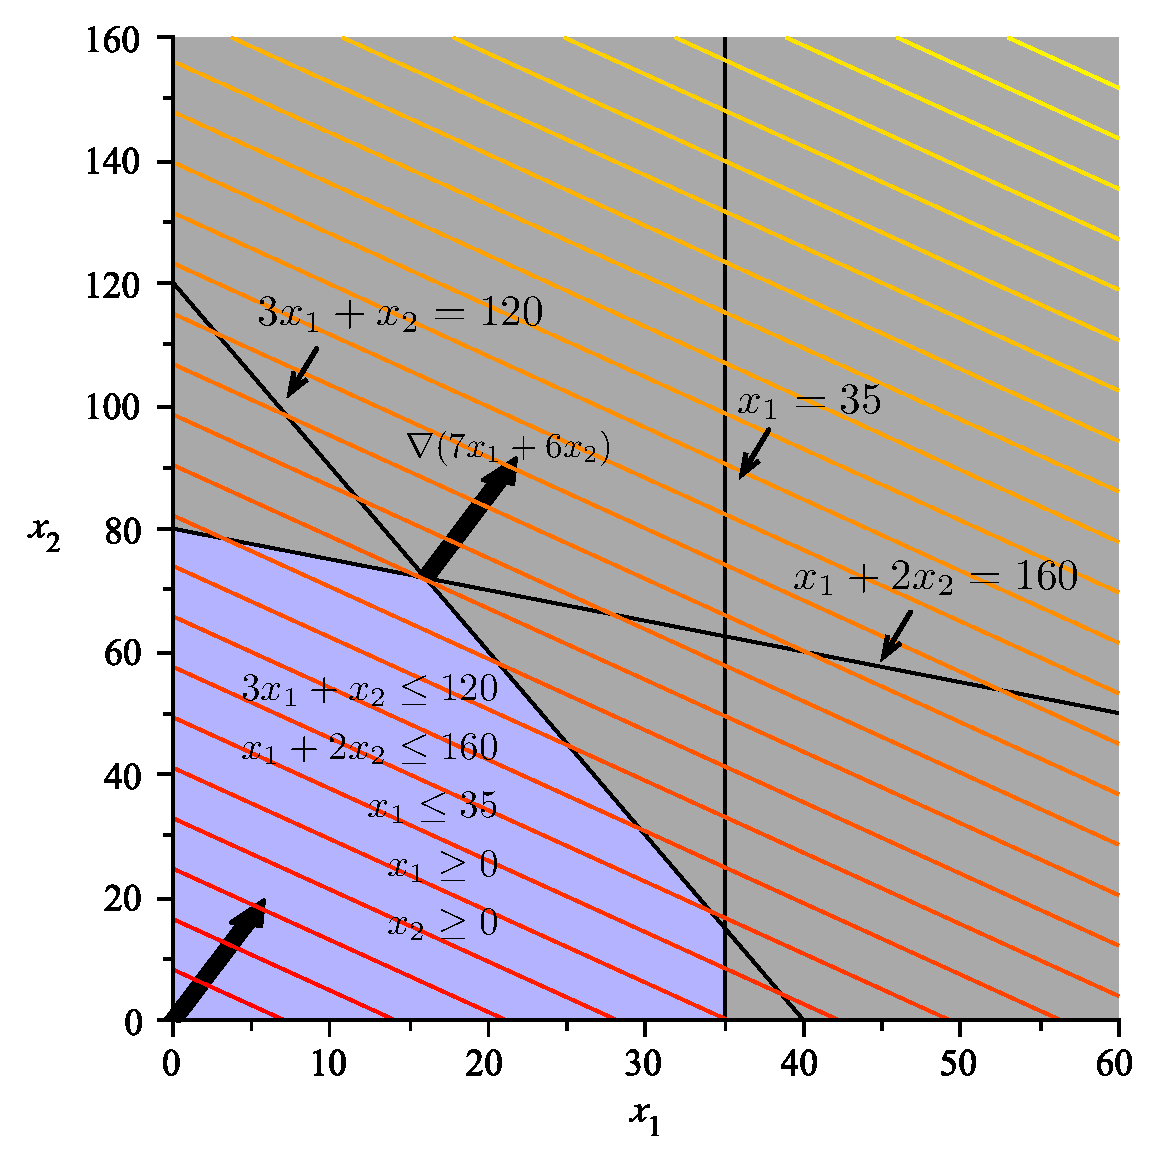
\includegraphics[scale=0.4]{FeasibleRegion.pdf}
%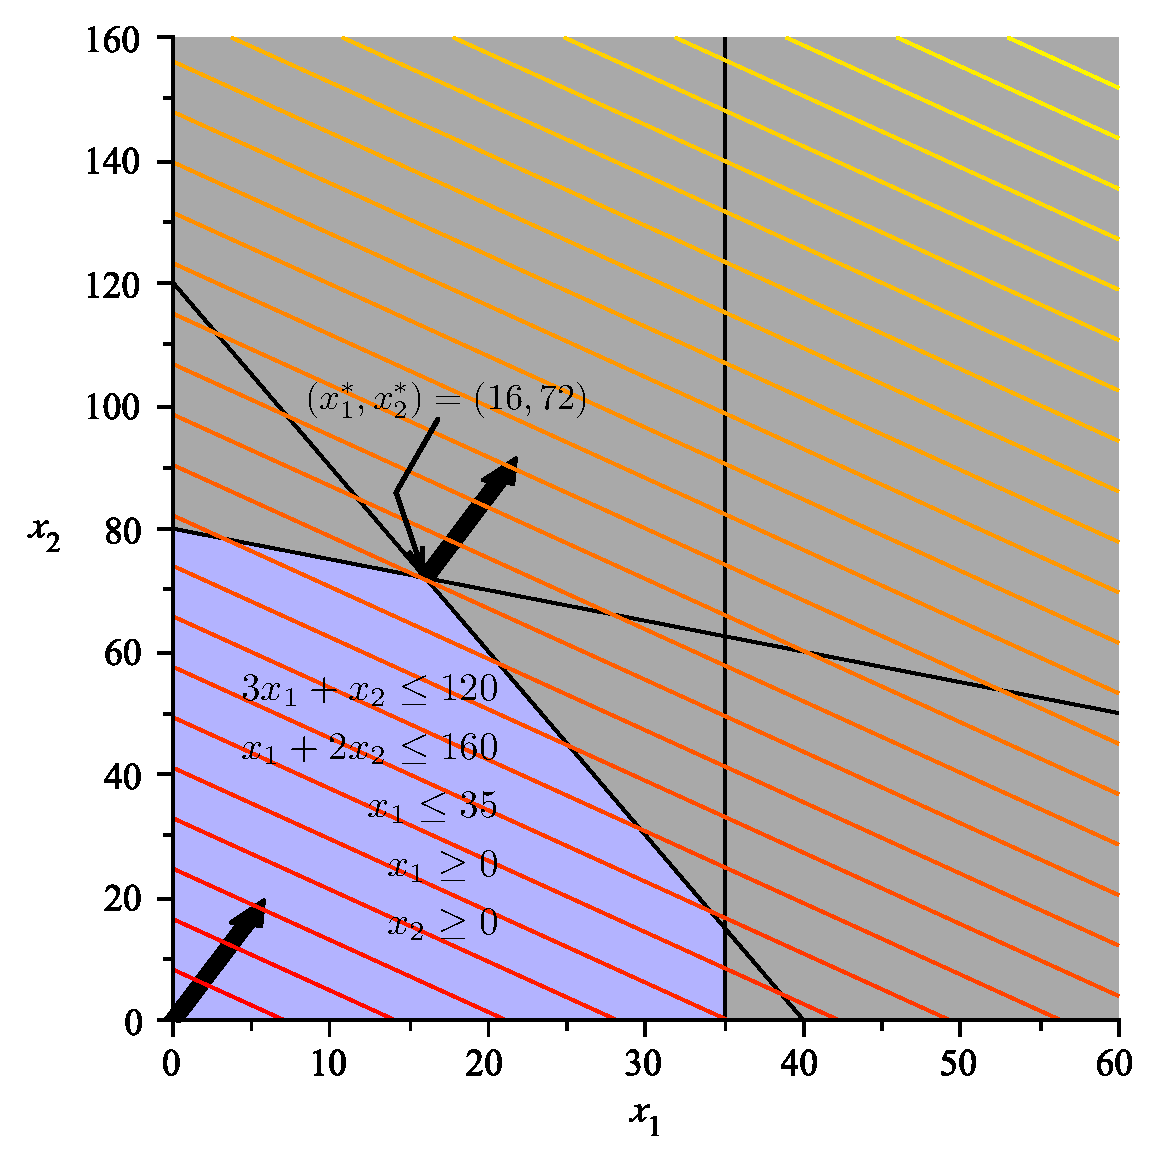
\includegraphics[scale=0.4]{FeasibleRegionWithMax.pdf}
\caption{Feasible Region and Level Curves of the Objective Function: The shaded region in the plot is the feasible region and represents the intersection of the five inequalities constraining the values of $x_1$ and $x_2$. On the right, we see the optimal solution is the ``last'' point in the feasible region that intersects a level set as we move in the direction of increasing profit.}
\label{fig:ToyExampleFeasibleRegion}
\end{figure}

\begin{example}{Continuation of ToyMaker Example}{}Let's continue the example of the Toy Maker begin in Example \ref{ex:ToyMaker}.  Solve this problem graphically.
\end{example}
\begin{solution} To solve the linear programming problem graphically, begin by drawing the feasible region. This is shown in the blue shaded region of Figure \ref{fig:ToyExampleFeasibleRegion}. 


After plotting the feasible region, the next step is to plot the level curves of the objective function. In our problem, the level sets will have the form:
\begin{displaymath}
7x_1 + 6x_2 = z \implies x_2 = \frac{-7}{6}x_1 + \frac{z}{6}
\end{displaymath}
This is a set of parallel lines with slope $-7/6$ and intercept $z/6$ where $z$ can be varied as needed. The level curves for various values of $z$ are parallel lines. In Figure \ref{fig:ToyExampleFeasibleRegion} they are shown in colors ranging from red to yellow depending upon the value of $z$. Larger values of $z$ are more yellow. 

To solve the linear programming problem, follow the level sets along the gradient (shown as the black arrow) until the last level set (line) intersects the feasible region. If you are doing this by hand, you can draw a single line of the form $7x_1 + 6x_2 = z$ and then simply draw parallel lines in the direction of the gradient $(7,6)$. At some point, these lines will fail to intersect the feasible region. The last line to intersect the feasible region will do so at a point that maximizes the profit. In this case, the point that maximizes $z(x_1,x_2) = 7x_1 + 6x_2$, subject to the constraints given, is $(x_1^*, x_2^*) = (16,72)$. 
\newpage
Note the point of optimality $(x_1^*, x_2^*) = (16,72)$ is at a corner of the feasible region. This corner is formed by the intersection of the two lines: $3x_1 + x_2 = 120$ and $x_1 + 2x_2 = 160$. In this case, the constraints 
\begin{gather*}
3x_1 + x_2 \leq 120\\
x_1 + 2x_2 \leq 160
\end{gather*}
are both \textit{binding}, while the other constraints are non-binding. In general, we will see that when an optimal solution to a linear programming problem exists, it will always be at the intersection of several binding constraints; that is, it will occur at a corner of a higher-dimensional polyhedron.  
\end{solution}

We can now define an algorithm for identifying the solution to a linear programing problem in two variables with a \textit{bounded} feasible region. 
\begin{algorithm}[H]
\captionsetup{labelformat=empty} % Disable numbering for this specific algorithm
%\caption{(First Try) Algorithm for Solving a Two Variable Linear Programming Problem Graphically--Bounded Feasible Region, Unique Solution Case}
\label{alg:GraphLPBoundedUniqueSoln}
\begin{center}
\begin{minipage}[t]{\textwidth-1em}
\underline{\textbf{(First Try) Algorithm for Solving a Linear Programming Problem Graphically}}\\
\textit{Bounded Feasible Region, Unique Solution}
\begin{enumerate*}
\item Plot the feasible region defined by the constraints.
\item Plot the level sets of the objective function.
\item For a maximization problem, identify the level set corresponding the greatest (least, for minimization) objective function value that intersects the feasible region. This point will be at a corner. 
\item The point on the corner intersecting the greatest (least) level set is a solution to the linear programming problem.  
\end{enumerate*}
\end{minipage}
\end{center}
\end{algorithm}

\begin{example}{Lemonade Vendor}{lemonadevendor}
Say you are a vendor of lemonade and lemon juice. Each unit of lemonade
requires 1 lemon and 2 litres of water. Each unit of lemon juice
requires 3 lemons and 1 litre of water. Each unit of lemonade gives a
profit of three dollars. Each unit of lemon juice gives a profit of two
dollars. You have 6 lemons and 4 litres of water available. How many
units of lemonade and lemon juice should you make to maximize profit?


If we let \(x\) denote the number of units of lemonade to be made and
let \(y\) denote the number of units of lemon juice to be made, then the
profit is given by \(3x + 2y\) dollars. We call \(3x + 2y\) the
objective function. Note that there are a number of constraints that
\(x\) and \(y\) must satisfied. First of all, \(x\) and \(y\) should be
nonnegative. The number of lemons needed to make \(x\) units of lemonade
and \(y\) units of lemon juice is \(x+3y\) and cannot exceed 6. The
number of litres of water needed to make \(x\) units of lemonade and
\(y\) units of lemon juice is \(2x+y\) and cannot exceed 4. Hence, to
determine the maximum profit, we need to maximize \(3x + 2y\) subject to
\(x\) and \(y\) satisfying the constraints \(x + 3y \leq 6\),
\(2x + y \leq 4\), \(x \geq 0\), and \(y \geq 0.\)


A more compact way to write the problem is as follows:
\[\begin{array}{rrcrll}
\mbox{maximize } & 3x & + & 2y & \\
\mbox{subject to} 
& x & + & 3y & \leq & 6 \\
& 2x & +&  y & \leq & 4 \\
& x &  & & \geq & 0 \\
& & & y & \geq & 0. \\
\end{array}\]

\end{example}
\begin{solution}
We can solve this maximization problem graphically as follows. We first
sketch the set of $(x,y)$  satisfying the
constraints, called the feasible region, on the \((x,y)\)-plane. We then
take the objective function \(3x+2y\) and turn it into an equation of a
line \(3x+2y = z\) where \(z\) is a parameter. Note that as the value of
\(z\) increases, the line defined by the equation \(3x+2y=z\) moves in
the direction of the normal vector
$(3,2)$ We call this direction the
direction of improvement. Determining the maximum value of the objective
function, called the optimal value, subject to the contraints amounts to
finding the maximum value of \(z\) so that the line defined by the
equation \(3x+2y=z\) still intersects the feasible region.






\begin{center}
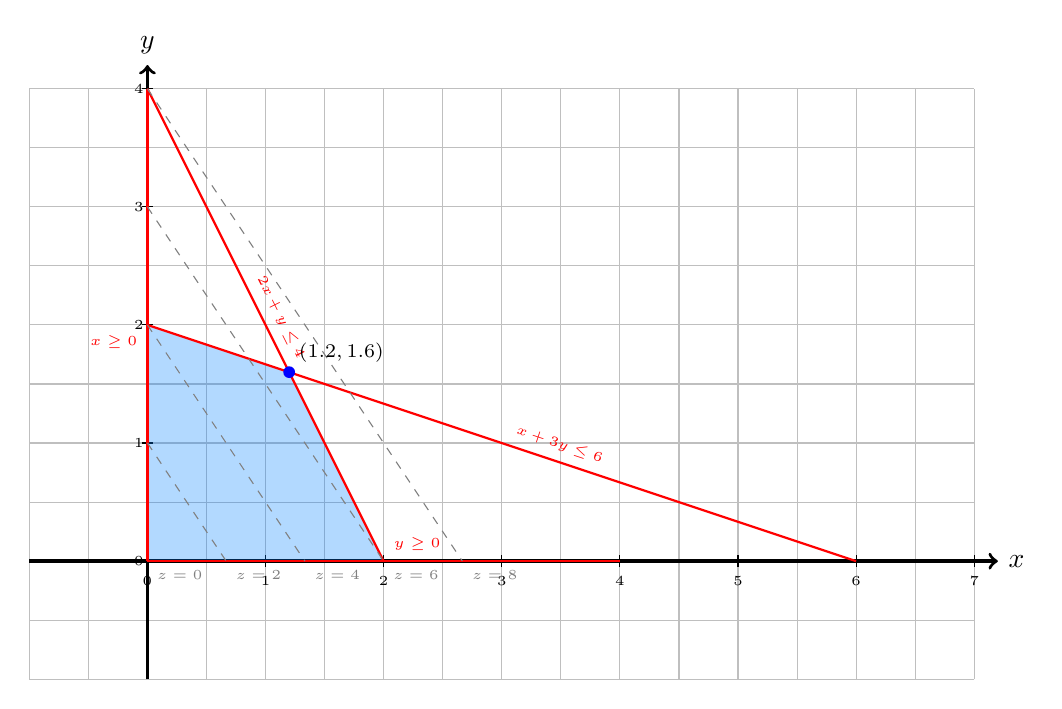
\begin{tikzpicture}[scale = 1.5]
    % Grid and axes
    \draw[gray!50, thin, step=0.5] (-1,-1) grid (7,4);
    \draw[very thick,->] (-1,0) -- (7.2,0) node[right] {$x$};
    \draw[very thick,->] (0,-1) -- (0,4.2) node[above] {$y$};

    % Axis labels
    \foreach \x in {0,...,7} \draw (\x,0.05) -- (\x,-0.05) node[below] {\tiny\x};
    \foreach \y in {0,...,4} \draw (-0.05,\y) -- (0.05,\y) node[left] {\tiny\y};

    % Shaded feasible region
    \fill[blue!50!cyan,opacity=0.3] (0,0) -- (0,2) -- (1.2,1.6) -- (2,0) -- cycle;

    % Constraint lines
    \draw[red,thick] (0,2) -- node[above right,sloped] {\tiny$x + 3y \leq 6$} (6,0);
    \draw[red,thick] (0,4) -- node[above,sloped] {\tiny$2x + y \leq 4$} (2,0);
    \draw[red,thick] (0,0) -- node[below left] {\tiny$x \geq 0$} (0,4);
    \draw[red,thick] (0,0) -- node[above right] {\tiny$y \geq 0$} (4,0);
    
        % Objective function contours
            \draw[dashed,gray] (0,4) -- (8/3,0) node[below right] {\tiny$z=8$};
    \draw[dashed,gray] (0,3) -- (2,0) node[below right] {\tiny$z=6$};
    \draw[dashed,gray] (0,2) -- (4/3,0) node[below right] {\tiny$z=4$};
    \draw[dashed,gray] (0,1) -- (2/3,0) node[below right] {\tiny$z=2$};
    \draw[dashed,gray] (0,0) -- (0,0) node[below right] {\tiny$z=0$};

    % Contour labels
    %\node[gray] at (0.5,3.5) {\tiny$3x + 2y = c$};
    
     \node[blue] at (1.2,1.6) [circle,fill,inner sep=1.5pt]{};

    % Labels for vertices
    \node[black,anchor=south west] at (1.2,1.6) {\scriptsize$(1.2,1.6)$};
\end{tikzpicture}
\end{center}


%\begin{tikzpicture}
%    \draw[gray!50, thin, step=0.5] (-1,-3) grid (5,4);
%    \draw[very thick,->] (-1,0) -- (5.2,0) node[right] {$x_1$};
%    \draw[very thick,->] (0,-3) -- (0,4.2) node[above] {$x_2$};
%
%    \foreach \x in {-1,...,5} \draw (\x,0.05) -- (\x,-0.05) node[below] {\tiny\x};
%    \foreach \y in {-3,...,4} \draw (-0.05,\y) -- (0.05,\y) node[right] {\tiny\y};
%
%    \fill[blue!50!cyan,opacity=0.3] (8/3,1/3) -- (1,2) -- (13/3,11/3) -- cycle;
%
%    \draw (-1,4) -- node[below,sloped] {\tiny$x_1+x_2\geq3$} (5,-2);
%    \draw (1,-3) -- (3,1) -- node[below left,sloped] {\tiny$2x_1-x_2\leq5$} (4.5,4);
%    \draw (-1,1) -- node[above,sloped] {\tiny$-x_1+2x_2\leq3$} (5,4);
%
%\end{tikzpicture}\footnote{
%\url{https://tex.stackexchange.com/questions/75933/how-to-draw-the-region-of-inequality}
%}
%
%\begin{center}
\includegraphics[width=0.8\linewidth]{images/lemon} \end{center}

In the figure above, the lines with \(z\) at 0, 4 and 6.8 have been
drawn. From the picture, we can see that if \(z\) is greater than 6.8,
the line defined by \(3x+2y = z\) will not intersect the feasible
region. Hence, the profit cannot exceed 6.8 dollars.

As the line \(3x+2y = 6.8\) does intersect the feasible region, \(6.8\)
is the maximum value for the objective function. Note that there is only
one point in the feasible region that intersects the line \(3x+2y=6.8\),
namely $(x,y) = (1.2,1.6)$.
In other words, to maximize profit, we want to make 1.2 units of
lemonade and 1.6 units of lemon juice.
\end{solution}





The example linear programming problem presented in this has a single optimal solution. In general, the following outcomes can occur in solving a linear programming problem: 
\begin{enumerate*}
\item The linear programming problem has a unique solution. (We've already seen this.)
\item There are infinitely many alternative optimal solutions.
\item There is no solution and the problem's objective function can grow to positive infinity for maximization problems (or negative infinity for minimization problems). 
\item There is no solution to the problem at all. 
\end{enumerate*}

Case 3 above can only occur when the feasible region is unbounded; that is, it cannot be surrounded by a ball with finite radius. We will illustrate each of these possible outcomes in the next four sections. We will prove that this is true in a later chapter.



\section{Infinitely Many Optimal Solutions}
\todoSection{ 20\% complete. Goal 80\% completion date: August 20\\
Notes: Need to work on this section.}
It can happen that there is more than one solution.  In fact, in this case, there are infinitly many optimal solutions.  
We'll study a specific linear programming problem with an infinite number of solutions by modifying the objective function in Example \ref{ex:ToyMaker}. 
\begin{example}{Toy Maker Alternative Solutions}{ex:ToyMakerAltOptSoln}
Suppose the toy maker in Example \ref{ex:ToyMaker} finds that it can sell planes for a profit of $\$18$ each instead of $\$7$ each. The new linear programming problem becomes:
\begin{equation}
\begin{aligned}
\max\;\;& z(x_1,x_2) = 18x_1 + 6x_2\\
s.t.\;\;&  3x_1 + x_2 \leq 120\\
& x_1 + 2x_2 \leq 160\\
& x_1 \leq 35\\
& x_1 \geq 0\\
& x_2 \geq 0
\end{aligned}.
\label{eqn:ToyMakerAltOptSoln}
\end{equation}
\end{example}

\begin{solution}
Applying our graphical method for finding optimal solutions to linear programming problems yields the plot shown in Figure \ref{fig:ToyMakerAltOptSoln}. The level curves for the function $z(x_1,x_2) = 18x_1 + 6x_2$ are \textit{parallel} to one face of the polygon boundary of the feasible region. Hence, as we move further up and to the right in the direction of the gradient (corresponding to larger and larger values of $z(x_1, x_2)$) we see that there is not \textit{one} point on the boundary of the feasible region that intersects that level set with greatest value, but instead a side of the polygon boundary described by the line $3x_1 + x_2 = 120$ where $x_1 \in [16, 35]$. 

Let:
\begin{displaymath}
P = \left\{(x_1,x_2) \ \  | \ \ \begin{array}{cc}3x_1 + x_2 \leq 120,\\ x_1 + 2x_2 \leq 160,\\ x_1 \leq 35,\\ x_1,x_2 \geq 0\end{array}  \right\}
\end{displaymath} 
that is, $P$ is the feasible region of the problem. Then for any value of $x_1^* \in [16,35]$ and any value $x_2^*$ so that  $3x_1^* + x_2^* = 120$, we will have $z(x_1^*, x_2^*) \geq z(x_1, x_2)$ for all $(x_1,x_2) \in P$. Since there are infinitely many values that $x_1$ and $x_2$  may take on, we see this problem has an infinite number of alternative optimal solutions.
\begin{figure}[H]
\centering
\begin{center}
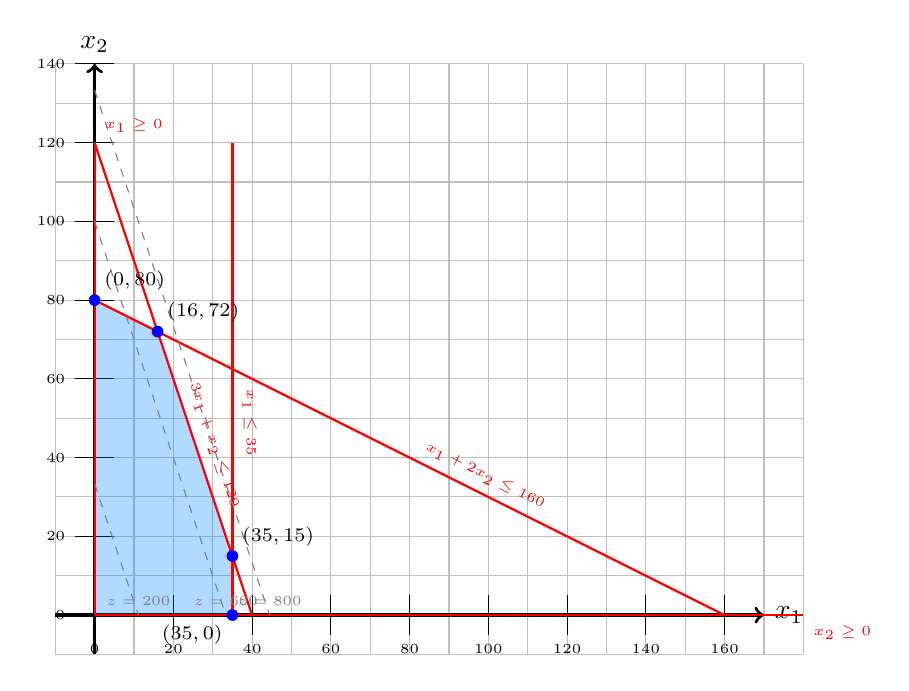
\begin{tikzpicture}[scale=0.05]
    % Grid and axes
    \draw[gray!50, thin, step=10] (-10,-10) grid (180,140);
    \draw[very thick,->] (-10,0) -- (170,0) node[right] {$x_1$};
    \draw[very thick,->] (0,-10) -- (0,140) node[above] {$x_2$};

    % Axis labels
    \foreach \x in {0,20,...,160} \draw (\x,5) -- (\x,-5) node[below] {\tiny\x};
    \foreach \y in {0,20,...,140} \draw (5,\y) -- (-5,\y) node[left] {\tiny\y};

    % Feasible region vertices
    \fill[blue!50!cyan,opacity=0.3] 
        (0,0) -- (0,80) -- (16,72) -- (35,15) -- (35,0) -- cycle;

    % Constraint lines

    \draw[red,thick] (0,120/1) --  node[above right, sloped] {\tiny $3x_1 + x_2 \leq 120$}(120/3,0);
    \draw[red,thick] (0,160/2) --  node[above right, sloped] {\tiny $x_1 + 2x_2 \leq 160$}(160,0);
    \draw[red,thick] (35,120) --  node[above right, sloped] {\tiny $x_1 \leq 35$}(35,0);
    \draw[red,thick] (0,0) -- (180,0) node[below right] {\tiny $x_2 \geq 0$};
    \draw[red,thick] (0,0) -- (0,120) node[above right] {\tiny $x_1 \geq 0$};

    % Objective function contours
    \draw[dashed,gray] (0,600/6) -- (600/18,0) node[above, sloped ] {\tiny $z = 600$};
    \draw[dashed,gray] (0,800/6) -- (800/18,0) node[above ] {\tiny $z = 800$};
    \draw[dashed,gray] (0,200/6) -- (200/18,0) node[above, sloped ] {\tiny $z = 200$};

    % Labels for vertices
    \node[blue] at (0,80) [circle,fill,inner sep=1.5pt]{};
    \node[blue] at (16,72) [circle,fill,inner sep=1.5pt]{};
    \node[blue] at (35,15) [circle,fill,inner sep=1.5pt]{};
    \node[blue] at (35,0) [circle,fill,inner sep=1.5pt]{};

    % Vertex coordinates
    \node[black,anchor=south west] at (0,80) {\scriptsize $(0,80)$};
    \node[black,anchor=south west] at (16,72) {\scriptsize $(16,72)$};
    \node[black,anchor=south west] at (35,15) {\scriptsize $(35,15)$};
    \node[black,anchor=north east] at (35,0) {\scriptsize $(35,0)$};

    % Objective function label
    %\node[gray] at (30,140) {\tiny $7x_1 + 6x_2 = z$};
\end{tikzpicture}
\end{center}
\caption{An example of infinitely many alternative optimal solutions in a linear programming problem. The level curves for $z(x_1,x_2) = 18x_1 + 6x_2$ are \textit{parallel} to one face of the polygon boundary of the feasible region. Moreover, this side contains the points of greatest value for $z(x_1,x_2)$ inside the feasible region. Any combination of $(x_1,x_2)$ on the line $3x_1 + x_2 = 120$ for $x_1 \in [16, 35]$ will provide the largest possible value $z(x_1,x_2)$ can take in the feasible region $S$.}
\label{fig:ToyMakerAltOptSoln}
\end{figure}
%\label{ex:ToyMakerAltOptSoln}
\end{solution}






%\begin{exercise}{}{} Use the graphical method for solving linear programming problems to solve the linear programming problem you defined in Exercise \ref{exer:ChemicalPlant}.
%\end{exercise}



Based on the example in this section, we can modify our algorithm for finding the solution to a linear programming problem graphically to deal with situations with an infinite set of alternative optimal solutions:
\begin{algorithm}[H]
\captionsetup{labelformat=empty} % Disable numbering for this specific algorithm

%\caption{Algorithm for Solving a Two Variable Linear Programming Problem Graphically--Bounded Feasible Region Case}
\label{alg:GraphLPBounded}
\begin{center}
\begin{minipage}[t]{\textwidth-1em}
\underline{\textbf{(Second try) Algorithm for Solving a Linear Programming Problem Graphically}}\\
\textit{Bounded Feasible Region}
\begin{enumerate*}
\item Plot the feasible region defined by the constraints.
\item Plot the level sets of the objective function.
\item For a maximization problem, identify the level set corresponding the greatest (least, for minimization) objective function value that intersects the feasible region. This point will be at a corner. 
\item The point on the corner intersecting the greatest (least) level set is a solution to the linear programming problem. 
\item \textbf{If the level set corresponding to the greatest (least) objective function value is parallel to a side of the polygon boundary next to the corner identified, then there are infinitely many alternative optimal solutions and any point on this side may be chosen as an optimal solution.} 
\end{enumerate*}
\end{minipage}
\end{center}
\end{algorithm}

\begin{learningcheckpoint}{How many optimal solutions?}{}
Consider the graphical representation below.  How many optimal solutions are there if we are maximizing?  How about if we are minimizing?
\begin{center}
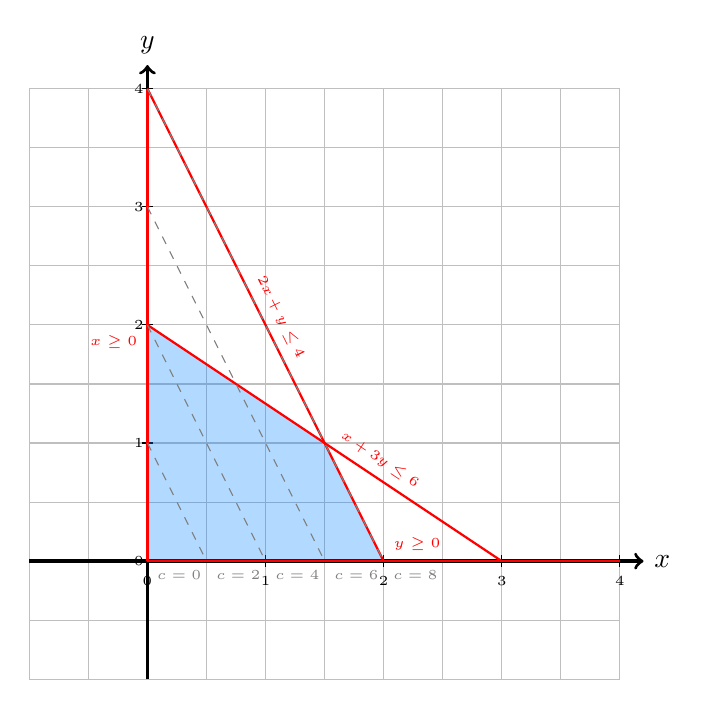
\begin{tikzpicture}[scale = 1.5]
    % Grid and axes
    \draw[gray!50, thin, step=0.5] (-1,-1) grid (4,4);
    \draw[very thick,->] (-1,0) -- (4.2,0) node[right] {$x$};
    \draw[very thick,->] (0,-1) -- (0,4.2) node[above] {$y$};

    % Axis labels
    \foreach \x in {0,...,4} \draw (\x,0.05) -- (\x,-0.05) node[below] {\tiny\x};
    \foreach \y in {0,...,4} \draw (-0.05,\y) -- (0.05,\y) node[left] {\tiny\y};

    % Shaded feasible region
    \fill[blue!50!cyan,opacity=0.3] (0,0) -- (0,2) -- (1.5,1) -- (2,0) -- cycle;

    % Constraint lines
    \draw[red,thick] (0,2) -- node[above right,sloped] {\tiny$x + 3y \leq 6$} (3,0);
    \draw[red,thick] (0,4) -- node[above,sloped] {\tiny$2x + y \leq 4$} (2,0);
    \draw[red,thick] (0,0) -- node[below left] {\tiny$x \geq 0$} (0,4);
    \draw[red,thick] (0,0) -- node[above right] {\tiny$y \geq 0$} (4,0);
    
        % Objective function contours
            \draw[dashed,gray] (0,4) -- (2,0) node[below right] {\tiny$c=8$};
    \draw[dashed,gray] (0,3) -- (1.5,0) node[below right] {\tiny$c=6$};
    \draw[dashed,gray] (0,2) -- (1,0) node[below right] {\tiny$c=4$};
    \draw[dashed,gray] (0,1) -- (0.5,0) node[below right] {\tiny$c=2$};
    \draw[dashed,gray] (0,0) -- (0,0) node[below right] {\tiny$c=0$};

    % Contour labels
    %\node[gray] at (0.5,3.5) {\tiny$3x + 2y = c$};
    
\end{tikzpicture}
\end{center}
\end{learningcheckpoint}

%\begin{exercise}{}{} Modify the linear programming problem from Exercise \ref{exer:ChemicalPlant} to obtain a linear programming problem with an infinite number of alternative optimal solutions. Solve the new problem and obtain a description for the set of alternative optimal solutions.\\
%
%\emph{[Hint: Just as in the example, $x_1$ will be bound between two value corresponding to a side of the polygon. Find those values and the constraint that is binding. This will provide you with a description of the form for any $x_1^* \in [a,b]$ and $x_2^*$ is chosen so that $cx_1^* + dx_2^* = v$, the point $(x_1^*, x_2^*)$ is an alternative optimal solution to the problem. Now you fill in values for $a$, $b$, $c$, $d$ and $v$.]}
%\end{exercise}

\section{Problems with No Solution} 
\todoSection{ 20\% complete. Goal 80\% completion date: August 20\\
Notes: Need to work on this section.}
Recall for \textit{any} mathematical programming problem, the feasible set or region is simply a subset of $\mathbb{R}^n$. If this region is empty, then there is no solution to the mathematical programming problem and the problem is said to be \textit{over constrained}. In this case, we say that the problem is \emph{infeasible}.  We illustrate this case for linear programming problems with the following example.
\begin{example}{Infeasible Problem}{}
 Consider the following linear programming problem:
\begin{equation}
\begin{aligned}
\max\;\;& z(x_1,x_2) = 3x_1 + 2x_2\\
s.t.\;\;&  \frac{1}{40}x_1 + \frac{1}{60}x_2 \leq 1\\
& \frac{1}{50}x_1 + \frac{1}{50}x_2 \leq 1\\
& x_1 \geq 30\\
& x_2 \geq 20
\end{aligned}
.
\label{eqn:LPInfeasible}
\end{equation}
\end{example}
\begin{solution}
The level sets of the objective and the constraints are shown in Figure \ref{fig:LPInfeasible}. 
\begin{figure}[H]
\centering
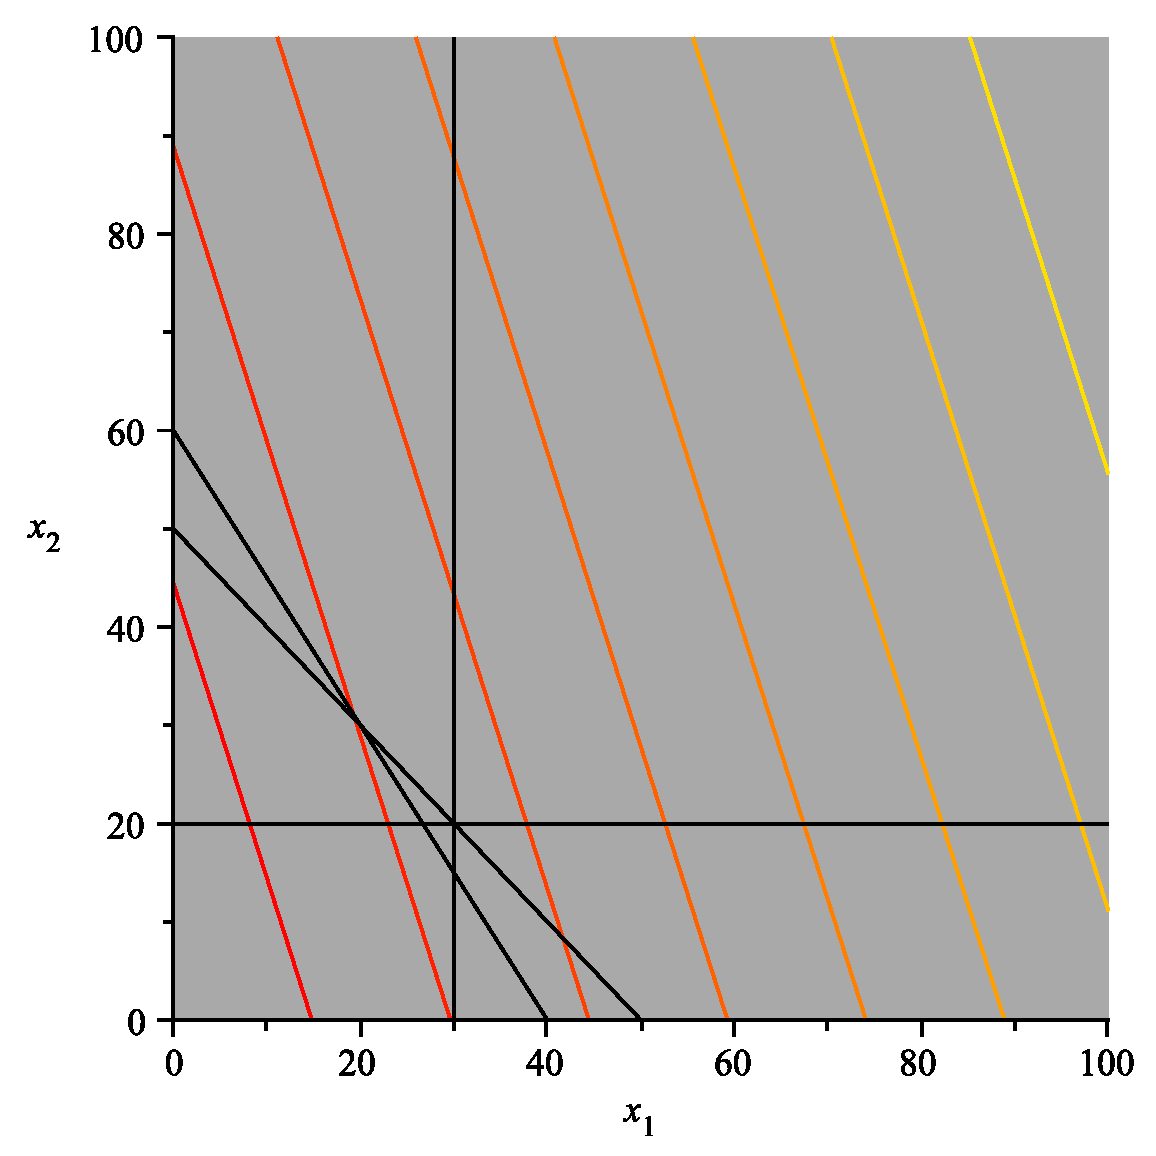
\includegraphics[scale=0.4]{LPNoSoln.pdf}
\caption{A Linear Programming Problem with no solution. The feasible region of the linear programming problem is empty; that is, there are no values for $x_1$ and $x_2$ that can simultaneously satisfy all the constraints. Thus, no solution exists.}
\label{fig:LPInfeasible}
\end{figure}

The fact that the feasible region is empty is shown by the fact that in Figure \ref{fig:LPInfeasible} there is no blue region--i.e., all the regions are gray indicating that the constraints are not satisfiable.
\label{ex:LPNoSoln}
\end{solution} 
Based on this example, we will modify our previous algorithm for finding the solution to linear programming problems graphically to consider the case that it is empty.  

Before stating complete algorithm, we also consider the unbounded case.

\section{Problems with Unbounded Feasible Regions}
\todoSection{ 20\% complete. Goal 80\% completion date: July 20\\
Notes: Need to work on this section.}
Consider the problem

\begin{align*}
\min \quad && z = 5x_1 + 7x_2  \\ 
\text{s.t.} \quad && x_1 + 3x_2 &\geq 6 \\ 
&& 5x_1 + 2x_2 &\geq 10 \\ 
&& x_2 &\leq 4 \\ 
&& x_1, x_2 &\geq 0 
\end{align*}



\begin{center}
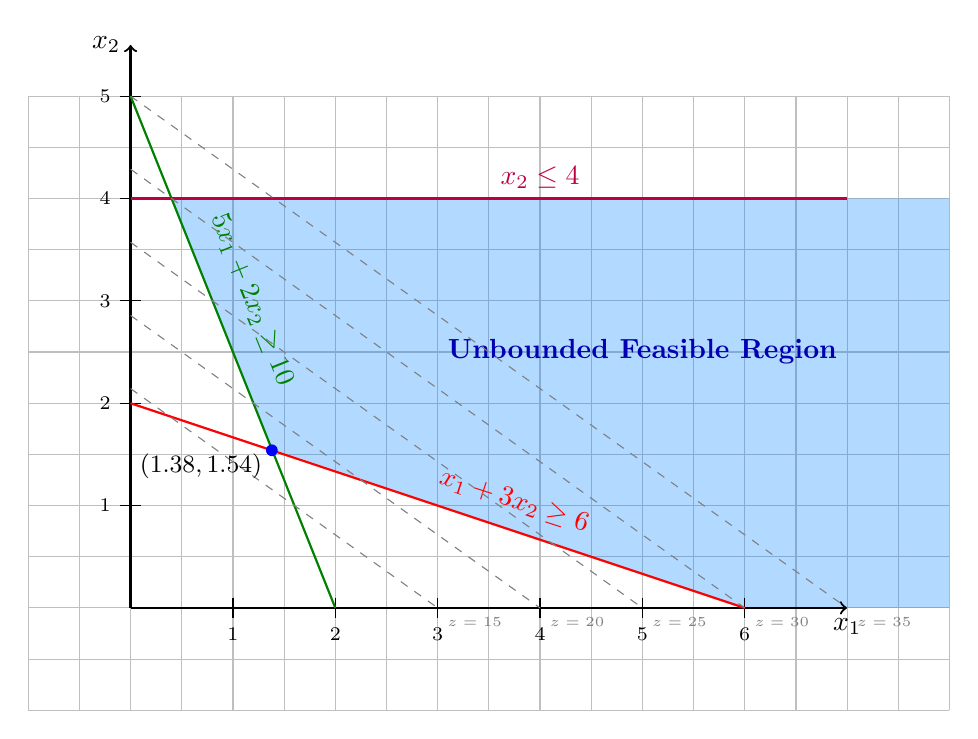
\begin{tikzpicture}[scale = 1.3]
    \draw[gray!50, thin, step=0.5] (-1,-1) grid (8,5);

    % Highlight the feasible region
    \fill[blue!50!cyan,opacity=0.3] 
        (0.4,4) -- (1.39,1.55)  -- (6,0) -- (8,0) -- (8,4) -- cycle;

    % Define axes
    \draw[thick,->] (0,0) -- (7,0) node[anchor=north] {$x_1$};
    \draw[thick,->] (0,0) -- (0,5.5) node[anchor=east] {$x_2$};

    % Add tick marks on the x_1-axis
    \foreach \x in {1,2,3,4,5,6} {
        \draw (\x,0.1) -- (\x,-0.1) node[anchor=north] {\scriptsize $\x$};
    }

    % Add tick marks on the x_2-axis
    \foreach \y in {1,2,3,4,5} {
        \draw (0.1,\y) -- (-0.1,\y) node[anchor=east] {\scriptsize $\y$};
    }

    % Define the constraints
    % Line 1: X + 3Y = 6
    \draw[red,thick] (0,2) -- (6,0);
    \node[red, rotate=-18, anchor=north west] at (3,1.5) {$x_1 + 3x_2 \geq 6$};

    % Line 2: 5X + 2Y = 10
    \draw[green!50!black,thick] (0,5) -- (2,0);
    \node[green!50!black, rotate=-68, anchor=north west] at (1,4) {$5x_1 + 2x_2 \geq 10$};

    % Line 3: Y = 4
    \draw[purple,thick] (0,4) -- (7,4);
    \node[purple, rotate=0, anchor=south] at (4,4) {$x_2 \leq 4$};

    % Label feasible region
    \node[blue!70!black, font=\bfseries] at (5,2.5) {Unbounded Feasible Region};

    % Mark intersection points
%    \fill[black] (0,4) circle (2pt) node[anchor=east] {\scriptsize $(0,4)$};
%    \fill[black] (6,0) circle (2pt) node[anchor=north] {\scriptsize $(6,0)$};

% Objective function contours
\foreach \c in {15,20,25,30,35} {
    \draw[dashed,gray] (0,\c/7) -- (\c/5,0) node[below right] {\tiny$z = \c$};
    }
%    \draw[dashed,gray] (0,3) -- (1.5,0) node[below right] {\tiny$c = 7.5$};
%    \draw[dashed,gray] (0,2) -- (1,0) node[below right] {\tiny$c = 5$};
%    \draw[dashed,gray] (0,1) -- (0.5,0) node[below right] {\tiny$c = 2.5$};
%    \draw[dashed,gray] (0,0) -- (0,0) node[below right] {\tiny$c = 0$};

    % Contour labels
    %\node[gray] at (0.5,3.5) {\tiny$3x_1 + 2x_2 = c$};
\node[blue,circle,fill,inner sep=1.5pt,label={[black,anchor=north east]\small$(1.38,1.54)$}] at (1.38,1.54) {};

\end{tikzpicture}
\end{center}

%\begin{center}
%%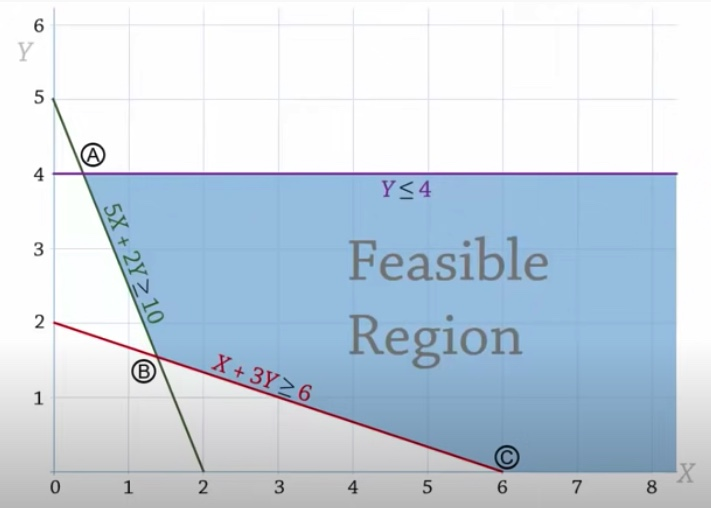
\includegraphics[scale = 0.4]{screenshots/example1-feasible-region}
%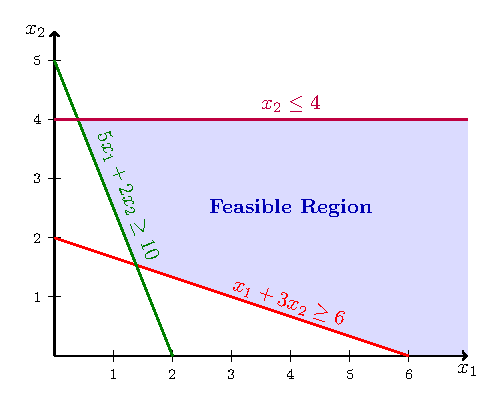
\includegraphics[scale = 1]{Figures/feasible-region-linear-ineqs}
%\end{center}

As you can see, the feasible region is \emph{unbounded}.  In particular, from any point in the feasible region, one can always find another feasible point by increasing the $X$ coordinate (i.e., move to the right in the picture).   However, this does not necessarily mean that the optimization problem is unbounded.

Indeed, the optimal solution is at $\mathbf{x}^* = (1.38, 1.54)$, the extreme point in the lower left hand corner, 
with optimal objective value
$$
z^* = 5 \cdot 1.38 + 7\cdot 1.54 = 17.7.
$$


%\begin{center}
%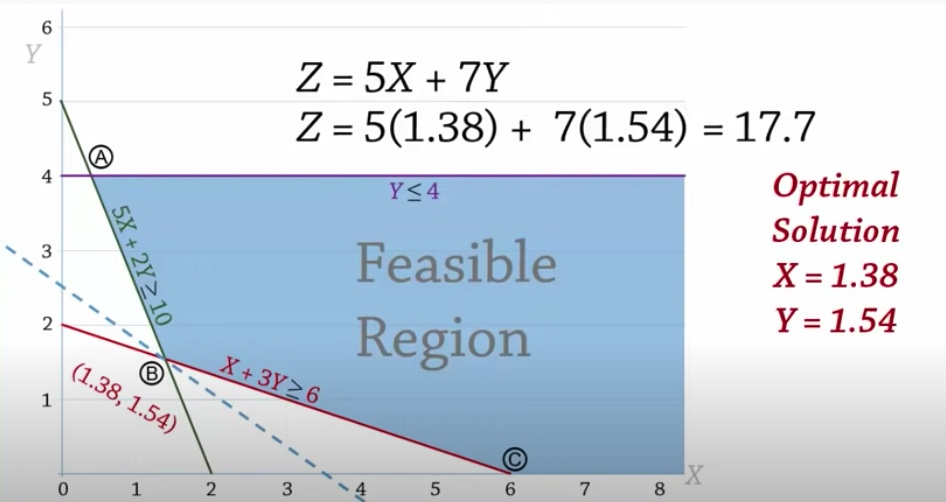
\includegraphics[scale = 0.4]{screenshots/example1-optimal-solution}
%\end{center}


Consider however, if we consider a different problem where we try to maximize the objective
\begin{align*}
{\color{red} \max }\quad && z = 5x_1 + 7x_2  \\ 
\text{s.t.} \quad && x_1 + 3x_2 &\geq 6 \\ 
&& 5x_1 + 2x_2 &\geq 10 \\ 
&& x_2 &\leq 4 \\ 
&& x_1, x_2 &\geq 0 
\end{align*}

\begin{solution}
This optimization problem is unbounded!  For example, notice that the point $(x_1,x_2) = (n,0)$ is feasible for all $n=1,2,3,\dots,$.   Then the objective function $z = 5n + 0$ follows the sequence $5, 10, 15, \dots,$, which diverges to infinity.   
\end{solution}


Let's see another example.

\begin{example}{}{} Consider the linear programming problem below:
\begin{equation}
\begin{aligned}
\max\;\;& z(x_1,x_2) = 2x_1 - x_2\\
s.t.\;\;& x_1 - x_2 \leq 1\\
& 2x_1 + x_2 \geq 6\\
&x_1,x_2 \geq 0
\end{aligned}
.
\label{eqn:LPUnboundFeasibleRegion1}
\end{equation}
\end{example}
\begin{solution}
The feasible region and level curves of the objective function are shown in Figure \ref{fig:LPUnboundFeasibleRegion1}. 
\begin{figure}[H]%[htbp]
\centering
\begin{center}
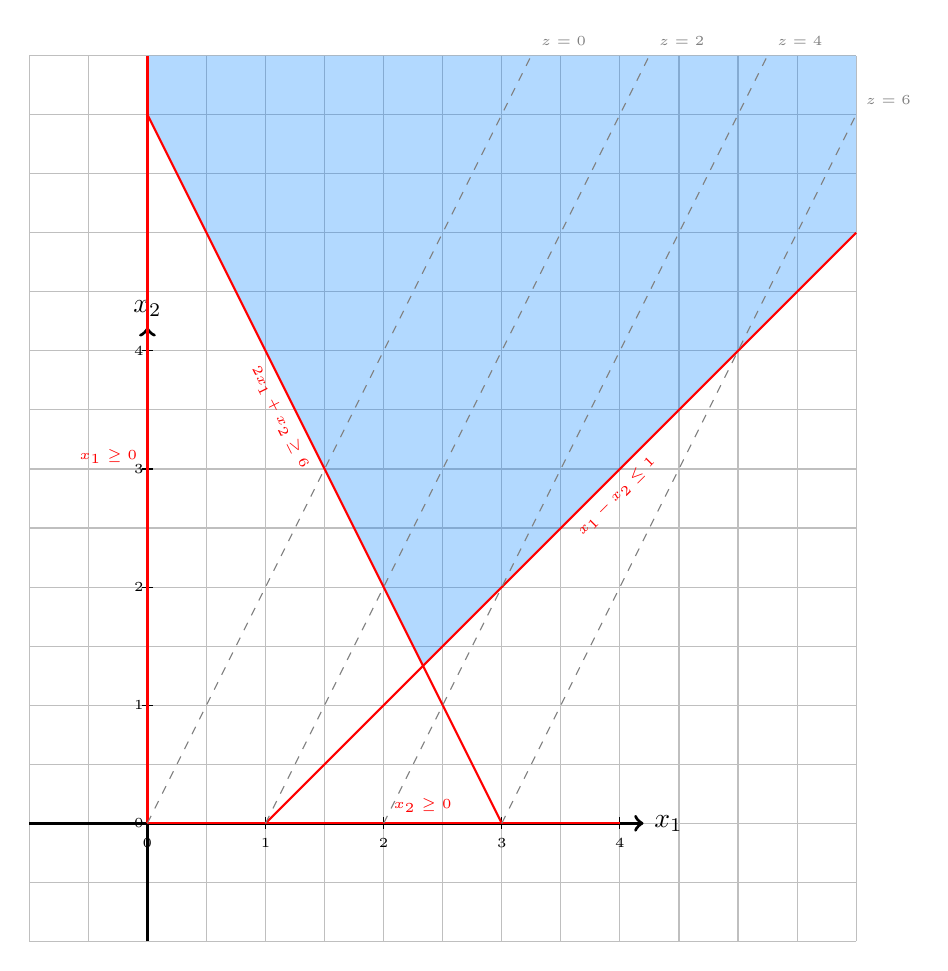
\begin{tikzpicture}[scale = 1.5]
    % Grid and axes
    \draw[gray!50, thin, step=0.5] (-1,-1) grid (6,6.5);
    \draw[very thick,->] (-1,0) -- (4.2,0) node[right] {$x_1$};
    \draw[very thick,->] (0,-1) -- (0,4.2) node[above] {$x_2$};

    % Axis labels
    \foreach \x in {0,...,4} \draw (\x,0.05) -- (\x,-0.05) node[below] {\tiny\x};
    \foreach \y in {0,...,4} \draw (-0.05,\y) -- (0.05,\y) node[left] {\tiny\y};

    % Shaded feasible region
    \fill[blue!50!cyan,opacity=0.3] (0,6.5) -- (0,6) -- (7/3, 4/3) -- (6,5) -- (6,6.5) -- cycle;

    % Constraint lines
    \draw[red,thick] (1,0) -- node[below right,sloped] {\tiny$x_1 - x_2 \leq 1$} (6,5);
    \draw[red,thick] (3,0) -- node[below left,sloped] {\tiny$2x_1 + x_2 \geq 6$} (0,6);
    \draw[red,thick] (0,0) -- node[below left] {\tiny$x_1 \geq 0$} (0,6.5);
    \draw[red,thick] (0,0) -- node[above right] {\tiny$x_2 \geq 0$} (4,0);

    % Objective function contours
   
    \draw[dashed,gray] (3,0) -- (6,6) node[above right] {\tiny$z=6$};
    \draw[dashed,gray] (2,0) -- (5.25,6.5) node[above right] {\tiny$z=4$};
    \draw[dashed,gray] (1,0) -- (4.25,6.5) node[above right] {\tiny$z=2$};
 \draw[dashed,gray] (0,0) -- (3.25,6.5) node[above right] {\tiny$z=0$};
    % Contour labels
    %\node[gray] at (2.5,3.5) {\tiny$2x_1 - x_2 = c$};

\end{tikzpicture}
\end{center}
%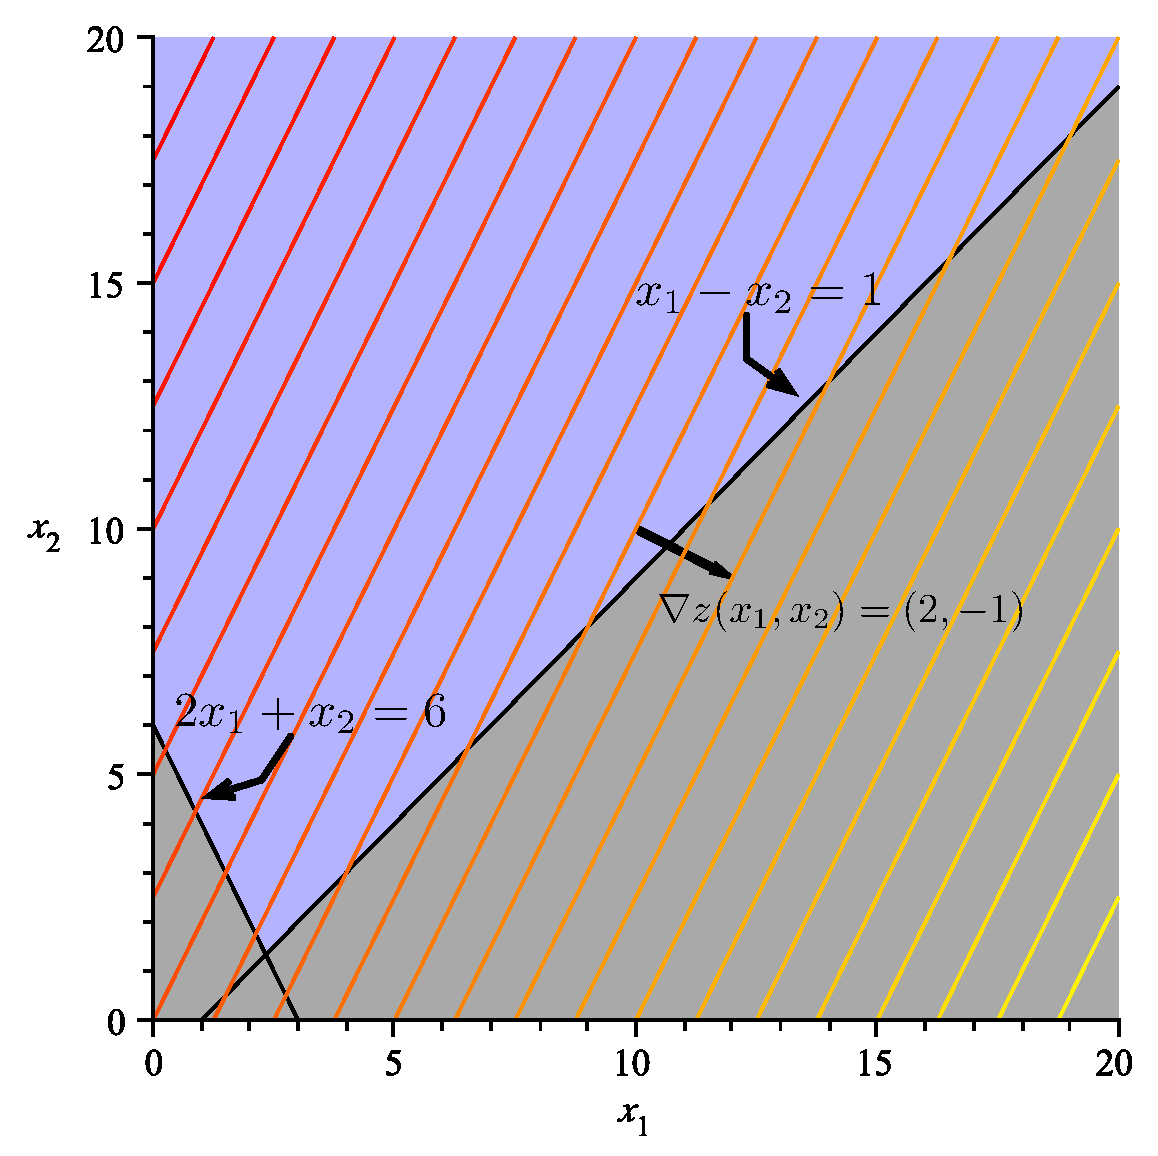
\includegraphics[scale=0.4]{UnboundedFeasibleRegion.pdf}
\caption{A Linear Programming Problem with Unbounded Feasible Region: Note that we can continue to make level curves of $z(x_1,x_2)$ corresponding to larger and larger values as we move down and to the right. These curves will continue to intersect the feasible region for any value of $v = z(x_1,x_2)$ we choose. Thus, we can make $z(x_1,x_2)$ as large as we want and still find a point in the feasible region that will provide this value. Hence, the optimal value of $z(x_1,x_2)$ subject to the constraints $+\infty$. That is, the problem is unbounded.}
\label{fig:LPUnboundFeasibleRegion1}
\end{figure}
The feasible region in Figure \ref{fig:LPUnboundFeasibleRegion1} is clearly unbounded since it stretches upward along the $x_2$ axis infinitely far and also stretches rightward along the $x_1$ axis infinitely far, bounded below by the line $x_1-x_2 = 1$. There is no way to enclose this region by a disk of finite radius, hence the feasible region is not bounded. 

We can draw more level curves of $z(x_1,x_2)$  in the direction of increase (down and to the right) as long as we wish. There will always be an intersection point with the feasible region because it is infinite. That is, these curves will continue to intersect the feasible region for any value of $v = z(x_1,x_2)$ we choose. Thus, we can make $z(x_1,x_2)$ as large as we want and still find a point in the feasible region that will provide this value. Hence, the largest value $z(x_1,x_2)$ can take when $(x_1,x_2)$ are in the feasible region is $+\infty$. That is, the problem is unbounded.
\label{ex:LPUnboundFeasibleRegion1}
\end{solution}

Just because a linear programming problem has an unbounded feasible region does not imply that there is not a finite solution. We illustrate this case by modifying example \ref{ex:LPUnboundFeasibleRegion1}. 

\begin{example}{Continuation of Example}{ex:LPUnboundFeasibleRegion2}
Consider the linear programming problem from Example \ref{ex:LPUnboundFeasibleRegion1} with the new objective function: $z(x_1,x_2) = (1/2)x_1 - x_2$. Then we have the new problem:
\begin{equation}
\begin{aligned}
\max\;\;&& z(x_1,x_2) =\frac{1}{2}x_1 - x_2\\
s.t.\;\;&& x_1 - x_2 &\leq 1\\
&& 2x_1 + x_2 &\geq 6\\
&&x_1,x_2 &\geq 0
\end{aligned}.
\label{eqn:LPUnboundFeasibleRegion2}
\end{equation}
\end{example}
\begin{solution}
The feasible region, level sets of $z(x_1,x_2)$ and gradients are shown in Figure \ref{fig:LPUnboundFeasibleRegion2}. In this case note, that the direction of increase of the objective function is \textit{away} from the direction in which the feasible region is unbounded (i.e., downward). As a result, the point in the feasible region with the largest $z(x_1,x_2)$ value is $(7/3,4/3)$. Again this is a vertex: the binding constraints are $x_1 - x_2 = 1$ and $2x_1 + x_2 = 6$ and the solution occurs at the point these two lines intersect.
\begin{figure}[H]%[htbp]
\begin{center}
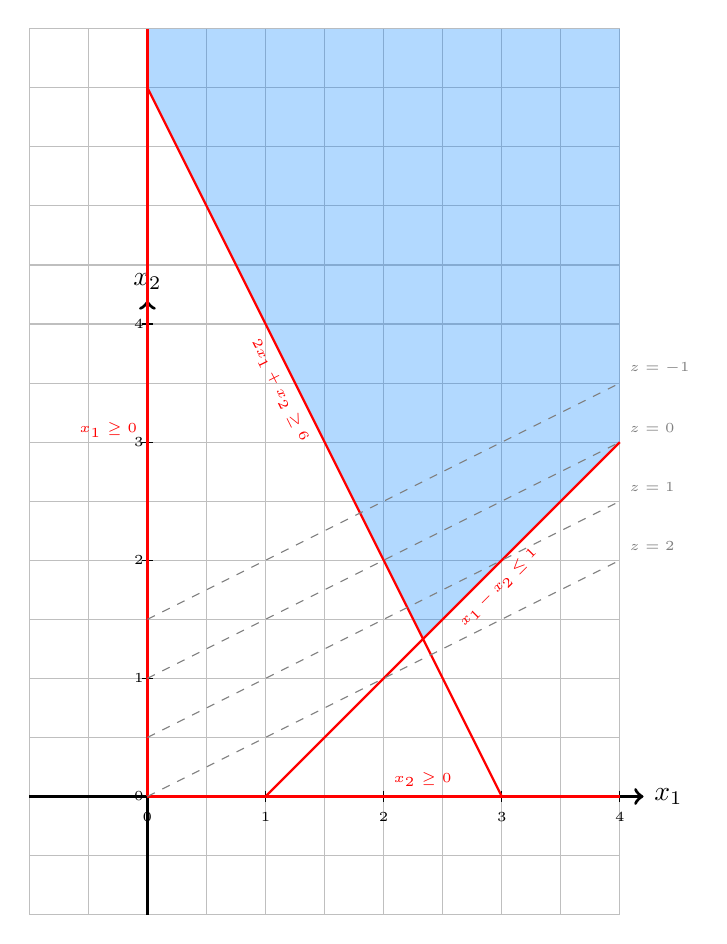
\begin{tikzpicture}[scale = 1.5]
    % Grid and axes
    \draw[gray!50, thin, step=0.5] (-1,-1) grid (4,6.5);
    \draw[very thick,->] (-1,0) -- (4.2,0) node[right] {$x_1$};
    \draw[very thick,->] (0,-1) -- (0,4.2) node[above] {$x_2$};

    % Axis labels
    \foreach \x in {0,...,4} \draw (\x,0.05) -- (\x,-0.05) node[below] {\tiny\x};
    \foreach \y in {0,...,4} \draw (-0.05,\y) -- (0.05,\y) node[left] {\tiny\y};

    % Shaded feasible region
    \fill[blue!50!cyan,opacity=0.3] (0,6.5) -- (0,6) -- (7/3, 4/3) -- (4,3) -- (4,6.5) -- cycle;

    % Constraint lines
    \draw[red,thick] (1,0) -- node[below right,sloped] {\tiny$x_1 - x_2 \leq 1$} (4,3);
    \draw[red,thick] (3,0) -- node[below left,sloped] {\tiny$2x_1 + x_2 \geq 6$} (0,6);
    \draw[red,thick] (0,0) -- node[below left] {\tiny$x_1 \geq 0$} (0,6.5);
    \draw[red,thick] (0,0) -- node[above right] {\tiny$x_2 \geq 0$} (4,0);

    % Objective function contours
    \draw[dashed,gray] (0,0) -- (4,2) node[above right] {\tiny$z=2$};
    \draw[dashed,gray] (0,0.5) -- (4,2.5) node[above right] {\tiny$z=1$};
    \draw[dashed,gray] (0,1) -- (4,3) node[above right] {\tiny$z=0$};
    \draw[dashed,gray] (0,1.5) -- (4,3.5) node[above right] {\tiny$z=-1$};

    % Contour labels
    %\node[gray] at (2.5,3.5) {\tiny$\frac{1}{2}x_1 - x_2 = c$};

\end{tikzpicture}
\end{center}

\centering
%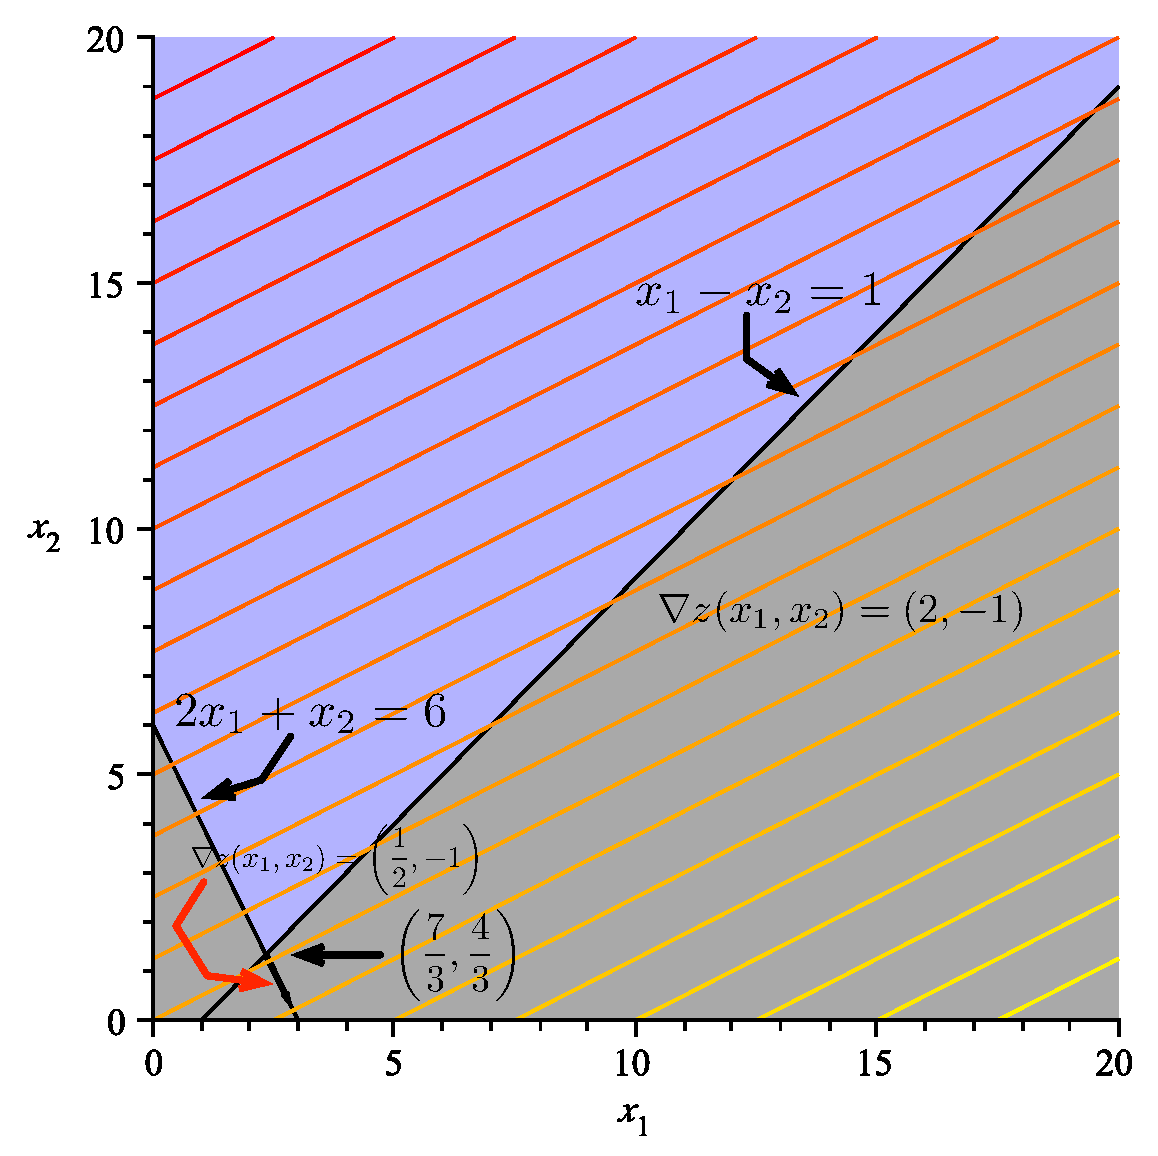
\includegraphics[scale=0.4]{UnboundedFeasibleRegionFiniteSolution.pdf}
\caption{A Linear Programming Problem with Unbounded Feasible Region and Finite Solution: In this problem, the level curves of $z(x_1,x_2)$ increase in a more ``southernly'' direction that in Example \ref{ex:LPUnboundFeasibleRegion2}--that is, \textit{away} from the direction in which the feasible region increases without bound. The point in the feasible region with largest $z(x_1,x_2)$ value is $(7/3,4/3)$. Note again, this is a vertex.}
\label{fig:LPUnboundFeasibleRegion2}
\end{figure}
\label{ex:LPUnboundFeasibleRegion2}
\end{solution}
Based on these two examples, we can modify our algorithm for graphically solving a two variable linear programming problems to deal with the case when the feasible region is unbounded.

\begin{algorithm}
\caption{Algorithm for Solving a Two-Variable Linear Programming Problem Graphically}
\label{alg:GraphLPGeneral}
\begin{enumerate}
    \item Plot the feasible region defined by the constraints.
    \item If the feasible region is empty, there is no solution.
    \item Plot the level sets of the objective function.
    \item \textbf{Bounded Case:}
    \begin{enumerate}
        \item Identify the corner point where the optimal level set (maximization: greatest; minimization: least) intersects the feasible region.
        \item If the level set is parallel to a side of the feasible region at this corner, any point on this side is an optimal solution (infinitely many solutions).
    \end{enumerate}
    \item \textbf{Unbounded Case:}
    \begin{enumerate}
        \item If the level sets intersect the feasible region indefinitely (maximization: larger; minimization: smaller), the problem is unbounded ($+\infty$ or $-\infty$).
        \item Otherwise, proceed as in the bounded case.
    \end{enumerate}
\end{enumerate}
\end{algorithm}


\newpage

\section{Exercises}\label{exercises}
%\addcontentsline{toc}{section}{Exercises}
\begin{ex}
Consider the following system of constraints:
\[
x + y \geq 5
\]
\[
x \geq 0, \quad y \geq 0
\]
Which of the following statements is true about the feasible region?
\begin{enumerate}
    \item  The feasible region is a bounded polygon.
    \item The feasible region is an unbounded region.
    \item The feasible region consists of a single point.
    \item The problem is infeasible.
\end{enumerate}


\end{ex}

\begin{ex} \label{ex:feasible-region}
Sketch all \(\begin{bmatrix} x \\ y \end{bmatrix}\) satisfying
\[
x - 2y \leq 2
\]
on the \((x,y)\)-plane.
\end{ex}

\begin{ex}{Graphically Solving}{}
Graph the feasible region of the linear program:
\begin{align*}
\min  \quad & x_1 - x_2\\
 & x_1 + x_2 \leq 6\\
 & x_1 - x_2 \geq 1\\
 & x_2 - x_1 \geq 3\\ 
 & x_1, x_2 \geq 0
\end{align*}
Without considering the objective function, how many feasible solutions are there?  Justify your answer.
\end{ex}


\begin{ex}{Graphical Method}{}
Use the graphical method to determine two optimal solutions to linear program:
\begin{align*}
\min  \quad& 3x_1 + 5x_2\\
 & 3x_1 + 2x_2 \ge 36\\
 & 6x_1 + 10x_2 \geq 90\\
 & x_1, x_2 \geq 0
\end{align*}
\end{ex}


\begin{ex}{}
\label{ex:infeasible}
Graph the feasible region of the linear program:
\begin{align*}
\min  \quad & x_1 - x_2\\
 & x_1 + x_2 \leq 6\\
 & x_1 - x_2 \geq 1\\
 & x_2 - x_1 \geq 3\\ 
 & x_1, x_2 \geq 0
\end{align*}
Without considering the objective function, how many feasible solutions are there?  Justify your answer.
\end{ex}





\begin{ex} \label{ex:lp-optimal-value}
Determine the optimal value of
\[
\begin{array}{rl}
\text{Minimize} & x + y \\
\text{Subject to} &  2x + y \geq 4 \\
& x + 3y \geq 1.
\end{array}
\]
\end{ex}

\begin{ex} \label{ex:lp-unbounded}
Show that the problem
\[
\begin{array}{rl}
\text{Minimize} & -x + y \\
\text{Subject to} &  2x - y \geq 0 \\
& x + 3y \geq 3
\end{array}
\]
is unbounded.
\end{ex}



\begin{ex}{}{} Does the following problem have a bounded solution? Why?
\begin{equation}
\begin{aligned}
\boldsymbol{\min}\;\;&& z(x_1,x_2) = 2x_1 - x_2\\
s.t.\;\;&& x_1 - x_2 &\leq 1\\
&& 2x_1 + x_2 &\geq 6\\
&&x_1,x_2 &\geq 0
\end{aligned}.
\end{equation}
[Hint: Use Figure \ref{fig:LPUnboundFeasibleRegion2} and Algorithm \ref{alg:GraphLPGeneral}.]
\label{exer:BoundedSolutionQuestion}
\end{ex}

\begin{ex}{}{} Modify the objective function in Example \ref{ex:LPUnboundFeasibleRegion1} to produce a problem with an infinite number of solutions. 
\end{ex}

\begin{ex}{}{} Modify the objective function in Exercise \ref{exer:BoundedSolutionQuestion} to produce a \textbf{minimization} problem that has a finite solution. Draw the feasible region and level curves of the objective to ``prove'' your example works. 

\emph{[Hint: Think about what direction of increase is required for the level sets of $z(x_1,x_2)$.]}
\end{ex}


\begin{ex}{}{} Consider the following problem:
\[
\begin{array}{rrcrll}
\mbox{minimize } & -2x_1 & + & x_2 & \\
\mbox{subject to} & -x_1 & + & x_2 & \leq & 3 \\
& x_1 & - & 2x_2 & \leq & 2 \\
& x_1 & & & \geq & 0 \\
& & & x_2 & \geq & 0. \\
\end{array}
\]

\begin{enumerate}
\item Show that for any \(t \geq 0\),
\[
\begin{bmatrix} x_1 \\ x_2 \end{bmatrix} = \begin{bmatrix} t \\ t \end{bmatrix}
\]
satisfies all the constraints. Show that the objective function is unbouned for this point as $t \to \infty$.

\item Show that \[
\begin{bmatrix} x_1 \\ x_2 \end{bmatrix} = \begin{bmatrix} 2t+2 \\ t \end{bmatrix}
\]
 is feasible for any \(t \geq 0\).  What is the objective function value at this point?  Show that the objective function is unbounded (yet again) by letting $t \to \infty$.
 \end{enumerate}
 \end{ex}
 
 \begin{ex}{}{} 
Consider the following problem:

\[
\begin{array}{rrcllll}
\mbox{maximize/minimize } & 2x & + & 2y \\
\mbox{subject to} & -x & + & 2y & \leq & 12 \\
& 2x & + & y & \geq & 4 \\
& x & + & 2y & \geq & 5 \\
& x & & & \geq & 0 \\
& & & y & \geq & 0. \\
\end{array}
\]

\begin{enumerate}

\item Determine the minimum value of \(2x + 2y\) by solving (graphically) the corresponding optimization problem. Show that the minimum is attained at a bounded feasible point.


\item Show that the maximum value of \(2x + 2y\) is unbounded by finding a feasible solution of the form
\[
\begin{bmatrix} x \\ y \end{bmatrix} = \begin{bmatrix} 5\\ 0\end{bmatrix} + t \begin{bmatrix} 1\\ 0\end{bmatrix}
\]
for any \(t \geq 0\). Show that as \(t \to \infty\), the objective function becomes unbounded.

\item Show that 
\[
\begin{bmatrix} x \\ y \end{bmatrix} = \begin{bmatrix} 0 \\ 6 \end{bmatrix} + t\begin{bmatrix} 1 \\ 2 \end{bmatrix}
\]
is feasible for any \(t \geq 0\). Compute the objective function value at this point and demonstrate that it is unbounded as \(t \to \infty\).


\end{enumerate}

\end{ex}

%By Kevin Cheung
%The book is licensed under the
%\href{http://creativecommons.org/licenses/by-sa/4.0/}{Creative Commons
%Attribution-ShareAlike 4.0 International License}.
%
%This file has been modified by Robert Hildebrand 2020.  
%CC BY SA 4.0 licence still applies.

%\section{Graphical example}\label{graphic}
%
%To motivate the subject of linear programming (LP), we begin with a
%planning problem that can be solved graphically.
%
%
%
%The above solution method can hardly be regarded as rigorous because we
%relied on a picture to conclude that \(3x + 2y \leq 6.8\) for all
%$(x,y)$ satisfying the constraints. But we
%can actually show this \emph{algebraically}.
%
%Note that multiplying both sides of the constraint \(x + 3y \leq 6\)
%gives \(0.2x + 0.6 y \leq 1.2\), and multiplying both sides of the
%constraint \(2x + y \leq 4\) gives \(2.8x + 1.4 y \leq 5.6\). Hence, any
%\(\begin{bmatrix} x\\y\end{bmatrix}\) that satisfies both \(x+3y\leq 6\)
%and \(2x+y \leq 4\) must also satisfy
%\((0.2x+0.6y) + (2.8x+1.4y) \leq 1.2 + 5.6\), which simplifies to
%\(3x + 2y \leq 6.8\) as desired! (Here, we used the fact that if
%\(a \leq b\) and \(c \leq d\), then \(a+c \leq b+d\).)
%
%Now, one might ask if it is always possible to find an algebraic proof
%like the one above for similar problems. If the answer is yes, how does
%one find such a proof? We will see answers to this question later on.
%
%Before we end this segment, let us consider the following problem:
%\[\begin{array}{rrcrll}
%\mbox{minimize } & -2x & + & y & \\
%\mbox{subject to} & -x & + & y & \leq & 3 \\
%& x & - &  2y & \leq & 2 \\
%& x &  & & \geq & 0 \\
%& & & y & \geq & 0. \\
%\end{array}\]
%
%Note that for any \(t \geq 0\),
%\(\begin{bmatrix} x \\ y\end{bmatrix} = \begin{bmatrix} t \\ t\end{bmatrix}\)
%satisfies all the constraints. The value of the objective function at
%\(\begin{bmatrix} x \\ y\end{bmatrix} = \begin{bmatrix} t \\ t\end{bmatrix}\)
%is \(-t\). As \(t \rightarrow \infty\), the value of the objective
%function tends to \(-\infty\). Therefore, there is no minimum value for
%the objective function. The problem is said to be unbounded. Later on,
%we will see how to detect unboundedness algorithmically.
%
%As an exercise, check that unboundedness can also be established by
%using
%\(\begin{bmatrix} x \\ y\end{bmatrix} = \begin{bmatrix} 2t+2 \\ t\end{bmatrix}\)
%for \(t \geq 0\).



\begin{ex} \label{ex:lp-diet-problem}
Suppose that you are shopping for dietary supplements to satisfy your
required daily intake of 0.40mg of nutrient \(M\) and 0.30mg of
nutrient \(N\). There are three popular products on the market. The
costs and the amounts of the two nutrients are given in the following
table:

\begin{table}[h!]
\centering
\begin{tabular}{lccc}
\toprule
         & Product 1 & Product 2 & Product 3 \\ \midrule
Cost     & \$27      & \$31      & \$24      \\
Daily amount of \(M\) & 0.16 mg   & 0.21 mg   & 0.11 mg   \\
Daily amount of \(N\) & 0.19 mg   & 0.13 mg   & 0.15 mg   \\ \bottomrule
\end{tabular}
\caption{Data for problem.}
\label{tab:your_table_label}
\end{table}

You want to determine how much of each product you should buy so that
the daily intake requirements of the two nutrients are satisfied at
minimum cost. Formulate your problem as a linear programming problem,
assuming that you can buy a fractional number of each product.
\end{ex}

\subsubsection*{Selected Solutions}
\label{solutions}
\addcontentsline{toc}{subsection}{Solutions}

\begin{solution}(Exercise~\ref{ex:inferasible})
In fact, constraints 2 and 3 point away from eachother, and hence there are no feasible solutions.  
\end{solution}


\begin{solution}(Exercise \ref{ex:feasible-region})

The points \((x,y)\) satisfying \(x-2y \leq 2\) are precisely those
above the line passing through \((2,0)\) and \((0,-1)\).
\end{solution}

\begin{solution}(\ref{ex:lp-optimal-value})

We want to determine the minimum value \(z\) so that \(x+y=z\) defines
a line that has a nonempty intersection with the feasible region.
However, we can avoid referring to a sketch by setting \(x=z-y\) and
substituting for \(x\) in the inequalities to obtain:

\begin{eqnarray*}
2(z-y) + y \geq 4 \\
(z-y) + 3y \geq 1,
\end{eqnarray*}

or equivalently,

\begin{eqnarray*}
z \geq 2+\frac{1}{2}y \\
z \geq 1-2y,
\end{eqnarray*}

Thus, the minimum value for \(z\) is
\(\min \{ 2+\frac{1}{2}y, 1-2y\}\), which occurs at
\(y = -\frac{2}{5}\). Hence, the optimal value is \(\frac{9}{5}\).

We can verify our work by doing the following. If our calculations
above are correct, then an optimal solution is given by
\(x = \frac{11}{5}\), \(y = -\frac{2}{5}\) since \(x = z - y\). It is
easy to check that this satisfies both inequalities and therefore is a
feasible solution.

Now, taking \(\frac{2}{5}\) times the first inequality and
\(\frac{1}{5}\) times the second inequality, we can infer the
inequality \(x+y \geq \frac{9}{5}\). The left-hand side of this
inequality is precisely the objective function. Hence, no feasible
solution can have objective function value less than \(\frac{9}{5}\).
But \(x = \frac{11}{5}\), \(y = -\frac{2}{5}\) is a feasible solution
with objective function value equal to \(\frac{9}{5}\). As a result,
it must be an optimal solution.

\textbf{Remark.} We have not yet discussed how to obtain the
multipliers \(\frac{2}{5}\) and \(\frac{1}{5}\) for inferring the
inequality \(x+y \geq \frac{9}{5}\). This is an issue that will be
taken up later. In the meantime, think about how one could have
obtained these multipliers for this particular exercise.
\end{solution}

\begin{solution}(Exercise \ref{ex:lp-unbounded})
We could glean some insight by first making a sketch on the
\((x,y)\)-plane.

The line defined by \(-x + y = z\) has \(x\)-intercept \(-z\). Note
that for \(z \leq -3\),
\(\begin{bmatrix} x\\y \end{bmatrix} = \begin{bmatrix} -z\\ 0\end{bmatrix}\)
satisfies both inequalities and the value of the objective function at
\(\begin{bmatrix} x\\y \end{bmatrix} = \begin{bmatrix} -z\\ 0\end{bmatrix}\)
is \(z\). Hence, there is no lower bound on the value of the objective
function.
\end{solution}

\begin{solution}(Exercise \ref{ex:lp-diet-problem})
Let \(x_i\) denote the amount of Product \(i\) to buy for
\(i = 1,2,3\). Then, the problem can be formulated as
\[
\begin{array}{rrcrcrll}
\mbox{minimize } & 27 x_1 & + & 31 x_2 & + & 24 x_3 \\
\mbox{subject to} 
& 0.16 x_1 & + & 0.21 x_2 & + & 0.11 x_3 & \geq & 0.30 \\
& 0.19 x_1 & + & 0.13 x_2 & + & 0.15 x_3 & \geq & 0.40 \\
& x_1 & , & x_2 & , & x_3 & \geq & 0. \\
\end{array}
\]

\textbf{Remark.} If one cannot buy fractional amounts of the products,
the problem can be formulated as
\[
\begin{array}{rrcrcrll}
\mbox{minimize } & 27 x_1 & + & 31 x_2 & + & 24 x_3 \\
\mbox{subject to} 
& 0.16 x_1 & + & 0.21 x_2 & + & 0.11 x_3 & \geq & 0.30 \\
& 0.19 x_1 & + & 0.13 x_2 & + & 0.15 x_3 & \geq & 0.40 \\
& x_1 & , & x_2 & , & x_3 & \geq & 0. \\
& x_1 & , & x_2 & , & x_3 & \in & \mathbb{Z}. \\
\end{array}
\]
\end{solution}


\section{Extreme Directions}

Let's define a procedure for finding the extreme directions, using the following LP's feasible region.  Graphically, we can see that the extreme directions should follow the the $s_1=0$ (red) line and the $s_3 = 0$ (orange) line. 
 
\begin{minipage}[t][][b]{.4\linewidth}
\begin{align*}
\mbox{max~~} & z = -5x_1 - x_2  \\\
\mbox{s.t.~~} & x_1 - 4x_2 +s_1 = 0  \\
& -x_1 + x_2 + s_2 = 1 \\
& -x_1 + 2x_2 +s_3 = 4 \\
& x_1, x_2, s_1, s_2, s_3 \ge 0.
\end{align*}
\end{minipage}%
\begin{minipage}[t][][b]{.6\linewidth}
\begin{center}  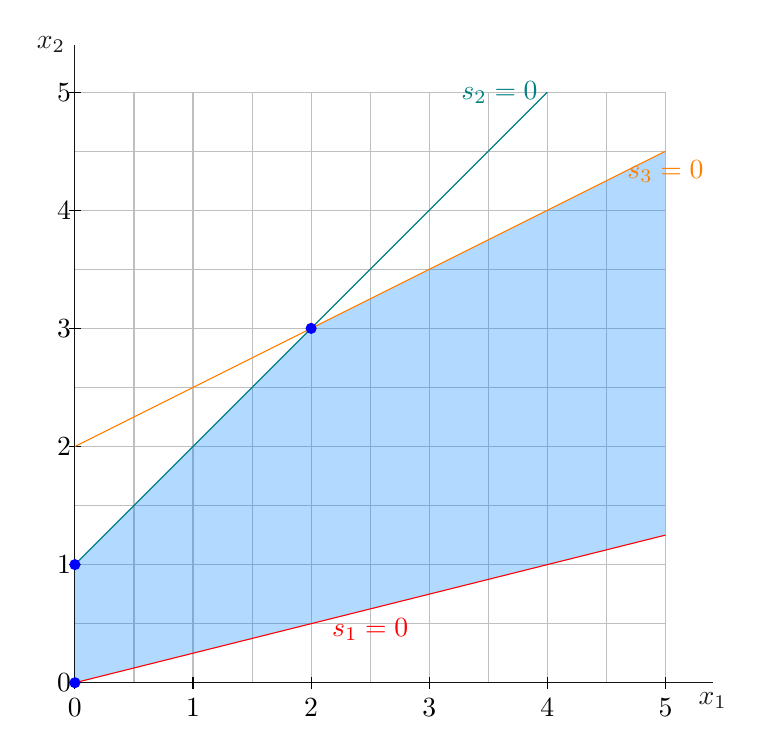
\begin{tikzpicture} [scale=1.5]
    \draw[gray!50, thin, step=.5] (0,0) grid (5,5);
    \draw[opacity=0.9] (0,0) -- (5.4,0) node[below] {$x_1$};
    \draw[opacity=0.9] (0,0) -- (0,5.4) node[left] {$x_2$}; % option \draw[very thick,->]

    \foreach \x in {0,...,5} \draw (\x,0.05) -- (\x,-0.05) node[below] {\x};
    \foreach \y in {0,...,5} \draw (-0.05,\y) -- (0.05,\y) node[left] {\y};

    \fill[blue!50!cyan,opacity=0.3] (0,0) -- (0,1) -- (2,3) -- (5,4.5) --(5,1.25)-- cycle;

    \draw [red](0,0) -- node[below] {$s_1=0$} (5, 1.25);
    \draw [teal] (0,1)  --  (4,5) node[left, sloped] {$s_2=0$};
    \draw [orange](0,2) --  (5,4.5) node[below, sloped] {$s_3=0$}; %node[above right ,sloped] 
    
    \node[fill=blue,circle,inner sep=0.05cm] at (0,0) {};
\node[fill=blue,circle,inner sep=0.05cm] at (0,1) {};
\node[fill=blue,circle,inner sep=0.05cm] at (2,3) {};

%	\filldraw[fill=red] (-0.05,-0.05) rectangle (0.05,0.05);
%	\filldraw[fill=red] (-0.05,.95) rectangle (0.05,1.05);
%	\filldraw[fill=red] (1.95,2.95) rectangle (2.05,3.05);
\end{tikzpicture} \end{center} 
\end{minipage}

\begin{center}  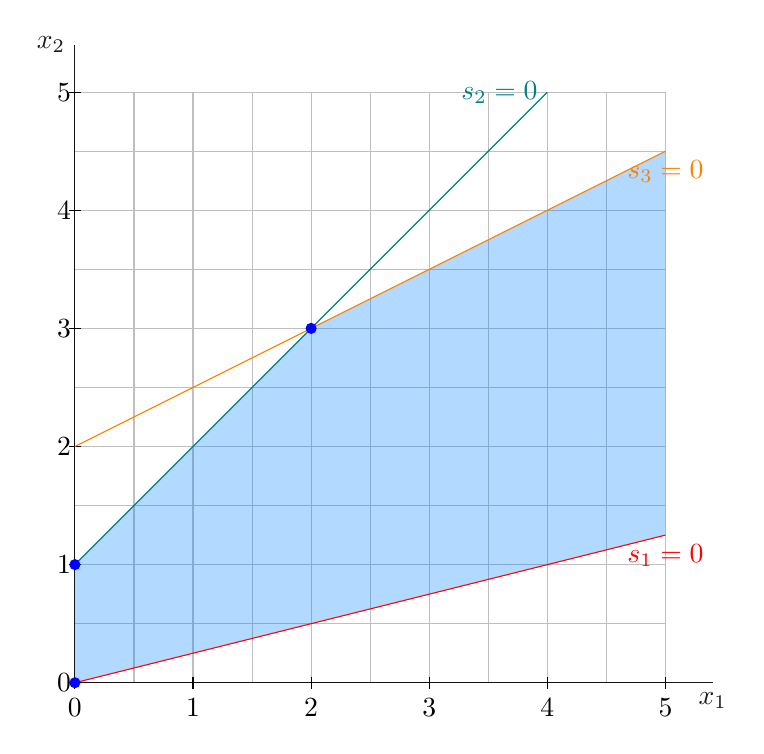
\begin{tikzpicture} [scale=1.5]
    \draw[gray!50, thin, step=.5] (0,0) grid (5,5);
    \draw[opacity=0.9] (0,0) -- (5.4,0) node[below] {$x_1$};
    \draw[opacity=0.9] (0,0) -- (0,5.4) node[left] {$x_2$}; % option \draw[very thick,->]

    \foreach \x in {0,...,5} \draw (\x,0.05) -- (\x,-0.05) node[below] {\x};
    \foreach \y in {0,...,5} \draw (-0.05,\y) -- (0.05,\y) node[left] {\y};

    \fill[blue!50!cyan,opacity=0.3] (0,0) -- (0,1) -- (2,3) -- (5,4.5) --(5,1.25)-- cycle;

\draw[domain=0:4,smooth,variable=\x, teal] plot ({\x},{\x+1}) node[left] {$s_2=0$};
\draw[domain=0:5,smooth,variable=\x, red] plot ({\x},{\x*1/4}) node[below] {$s_1=0$};
%    \draw [red](0,0) -- node[below] {$s_1=0$} (5, 1.25);
    %\draw [teal] (0,1)  --  (4,5) node[left, sloped] {$s_2=0$};
    \draw [orange](0,2) --  (5,4.5) node[below, sloped] {$s_3=0$}; %node[above right ,sloped] 
    \node[fill=blue,circle,inner sep=0.05cm] at (0,0) {};
\node[fill=blue,circle,inner sep=0.05cm] at (0,1) {};
\node[fill=blue,circle,inner sep=0.05cm] at (2,3) {};

%	\filldraw[fill=red] (-0.05,-0.05) rectangle (0.05,0.05);
%	\filldraw[fill=red] (-0.05,.95) rectangle (0.05,1.05);
%	\filldraw[fill=red] (1.95,2.95) rectangle (2.05,3.05);
\end{tikzpicture} \end{center} 

% \draw[scale=0.5,domain=-3:3,smooth,variable=\x,blue] plot ({\x},{\x*\x});


\medskip E.g., consider the $s_3=0$ (orange) line, to find the extreme direction start at extreme point (2,3) and find another feasible point on the orange line, say (4,4) and subtract (2,3) from (4,4), which yields (2,1). 

\medskip This is related to the slope in two-dimensions, as discussed in class, the rise is 1 and the run is 2. So this direction has a slope of 1/2, but this does not carry over easily to higher dimensions where directions cannot be defined by a single number. 

\medskip To find the extreme directions we can change the right-hand-side to $\mathbf{b} = \mathbf{0}$, which forms a polyhedral cone (in yellow), and then add the constraint $x_1 + x_2 = 1$. The intersection of the cone and  $x_1 + x_2 = 1$ form a line segment.

\begin{minipage}[t][][b]{.4\linewidth} \vspace{0mm}
\begin{align*}
\mbox{max~~} & z = -5x_1 - x_2  \\
\mbox{s.t.~~} & x_1 - 4x_2 +s_1 = 0  \\
& -x_1 + x_2 + s_2 = 0 \\
& -x_1 + 2x_2 +s_3 = 0 \\
& x_1 + x_2 = 1 \\
& x_1, x_2, s_1, s_2, s_3 \ge 0.
\end{align*}
\end{minipage}%
\begin{minipage}[t][][b]{.6\linewidth}
\begin{center} 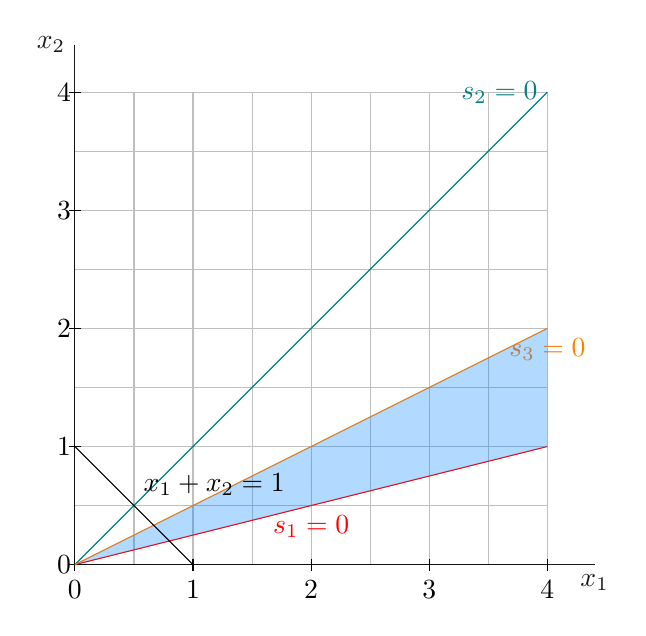
\begin{tikzpicture} [scale=1.5]
\draw[gray!50, thin, step=.5] (0,0) grid (4,4);
\draw[opacity=0.9] (0,0) -- (4.4,0) node[below] {$x_1$};
\draw[opacity=0.9] (0,0) -- (0,4.4) node[left] {$x_2$}; % option \draw[very thick,->]

\foreach \x in {0,...,4} \draw (\x,0.05) -- (\x,-0.05) node[below] {\x};
\foreach \y in {0,...,4} \draw (-0.05,\y) -- (0.05,\y) node[left] {\y};
        
\draw [red](0, 0) -- node[below] {$s_1=0$} (4, 1);
\draw [teal] (0,0)  -- (4,4) node[left, sloped] {$s_2=0$};
\draw [orange](0,0) -- (4,2) node[below, sloped] {$s_3=0$}; 
\fill[blue!50!cyan,opacity=0.3] (0,0) -- (4,2) -- (4,1) --  cycle; % \draw [orange!50!blue] 

\draw [black] (0,1)  -- node[above right] {$x_1+x_2 = 1$} (1,0); 
\end{tikzpicture} \end{center} 
\end{minipage}



\begin{center} 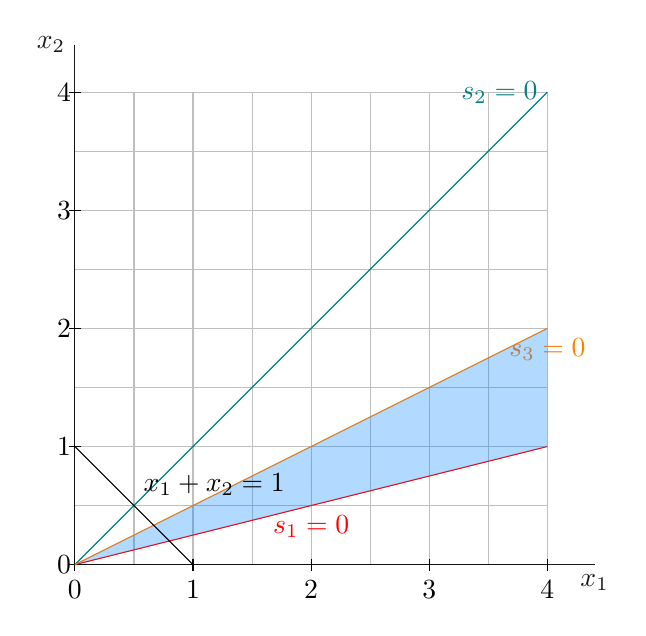
\begin{tikzpicture} [scale=1.5]
\draw[gray!50, thin, step=.5] (0,0) grid (4,4);
\draw[opacity=0.9] (0,0) -- (4.4,0) node[below] {$x_1$};
\draw[opacity=0.9] (0,0) -- (0,4.4) node[left] {$x_2$}; % option \draw[very thick,->]

\foreach \x in {0,...,4} \draw (\x,0.05) -- (\x,-0.05) node[below] {\x};
\foreach \y in {0,...,4} \draw (-0.05,\y) -- (0.05,\y) node[left] {\y};
        
\draw [red](0, 0) -- node[below] {$s_1=0$} (4, 1);
\draw [teal] (0,0)  -- (4,4) node[left, sloped] {$s_2=0$};
\draw [orange](0,0) -- (4,2) node[below, sloped] {$s_3=0$}; 
\fill[blue!50!cyan,opacity=0.3] (0,0) -- (4,2) -- (4,1) --  cycle; % \draw [orange!50!blue] 

\draw [black] (0,1)  -- node[above right] {$x_1+x_2 = 1$} (1,0); 
\end{tikzpicture} \end{center} 


\medskip Magnifying for clarity, and removing the $s_2=0$ (teal) line, as it is redundant, and marking the extreme points of the new feasible region, (4/5, 1/5) and (2/3, 1/3), with red boxes, we have:

\begin{center}  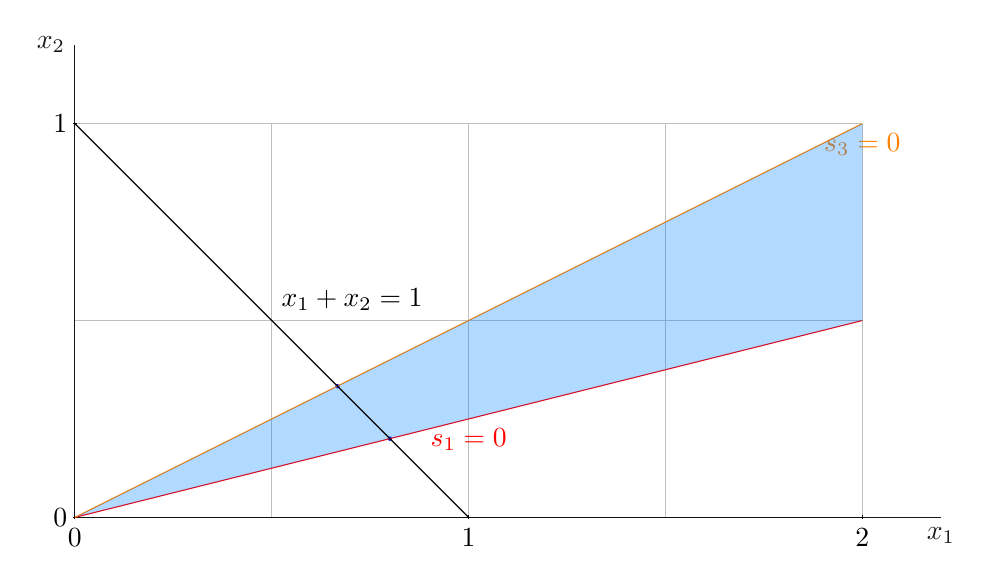
\begin{tikzpicture} [x=50mm, y=50mm] [scale=1.5]
\draw[gray!50, thin, step=.5] (0,0) grid (2,1);
\draw[opacity=0.9] (0,0) -- (2.2,0) node[below] {$x_1$};
\draw[opacity=0.9] (0,0) -- (0,1.2) node[left] {$x_2$}; % option \draw[very thick,->]

\foreach \x in {0,...,2} \draw (\x,0.005) -- (\x,-0.005) node[below] {\x};
\foreach \y in {0,...,1} \draw (-0.005,\y) -- (0.005,\y) node[left] {\y};

%\filldraw[fill=red] (0.8-0.02,0.2-0.02) rectangle (0.8+0.02,0.2+0.02);
%\filldraw[fill=red] (0.667-0.02,0.333-0.02) rectangle (0.667+0.02,0.333+0.02);
\node[fill=blue,circle,inner sep=0.02cm] at (0.8,0.2) {};
\node[fill=blue,circle,inner sep=0.02cm] at (0.667,0.333) {};


\draw [red](0, 0) -- node[below] {$s_1=0$} (2, .5);
\draw [orange](0,0) -- (2,1) node[below, sloped] {$s_3=0$}; 
\fill[blue!50!cyan,opacity=0.3] (0,0) -- (2,.5) -- (2,1) --  cycle; % \draw [orange!50!blue] 
\draw [black] (0,1)  -- node[above right] {$x_1+x_2 = 1$} (1,0); 
\end{tikzpicture} \end{center} 

The extreme directions are thus (4/5, 1/5) and (2/3, 1/3). \\



 
